{In this last chapter we are presenting the theory of Loop Quantum Gravity, which has to be regarded as a quantisation procedure which complies with all the fundamental traits of a relativistic theory, propounding a quantum model for the gravitational interaction. As a matter of fact, whether or not such a theory is the correct physical quantum interpretation of the gravitational field is something that should be decided by experiments, which are beyond our current capabilities. By the way, LQG widely inquires into the technicalities that a generally covariant quantum field theory should satisfy, which is an interesting issue, in general, even just from a mathematical point of view.}\, %Even if the spacetime of our physical world is $4$--dimensional, the theory does adapt to any dimension. It is for this reason that, in conclusion, I will discuss an attempt of a $3$--dimensional formulation of LQG, looking for some traits that can shed light on new aspects that may not be manifest in the original theory.


%$$\vdots$$
%Refer here to \cite{rov1}. Also \cite{pullin} and see Conclusion and Perspectives of LN3.

{\section{Quantisation of Holst theory}
  In this section, we are going to resume the ABI model and underscore again that quantum physical states shall be represented by functionals of gauge--classes of spatial spin connections in that. Next, we review some basics on the irreducible representations and the Haar metric  of the gauge group of the theory, and we construct the Hilbert space(s) of quantum states---by implementing covariance principles encoded in the boundary equations of the classical theory---and operators among them, which represent geometric observables of the gravitational field and which offer a beautiful geometrical quantum interpretation of space(time).}\\

%\subsection{Ashtekar--Barbero--Immirzi variables}
Gravitational Holst theory is modeled over the following principal structures %on the spacetime $\M^{1,3}$

\[\begin{tikzcd}
Q\arrow{r}{\iota} \arrow[swap]{d}{\SU(2)} & P\arrow{r}{\e}\arrow[swap]{d}{\SL(2,\C)}&L\M\arrow[swap]{d}{\GL_4}\\
\M^{1,3}\arrow{r} & \M^{1,3}\arrow{r} &\M^{1,3}\\
\end{tikzcd}
\]
{Holst--formulation perfectly fits with Yang--Mills quantisation, being a gravitational gauge--natural $\SL(2,\C)$--theory with fundamental fields $\left(e^I_\mu,\omega^{IJ}_\mu\right)\in\mathcal{F}(P)\times_\M\Con(P)$. Along the whole previous chapter, such dynamical variables were changed in $(e^I,\A^i,\kappa^i)$ and the $\Spin(1,3)$--connection $\omega^{IJ}$ was \emph{projected} on a $\SU(2)$--subbundle to the so--called Barbero--Immirzi connection $\A^i$, the difference being parametrized by $\kappa^i$. After adapting them to a Cauchy--bubble $(\Dd,\zeta,\imath)$ in order to evince bulks and gauge fields, we ended up with a pair of conjugated fields on a space--like $\Sigma^3\hookrightarrow\M^{1,3}$ of the form $\A^i_a,\E^b_j$, so--called 
\emph{Ashtekar connection} and \emph{Ashtekar electric field}, satisfying
$$\{\A^i_b(k),\E^b_j(k')\}=\beta\,\delta^i_j\delta^b_a\,\delta^{(3)}(k-k')
\qquad \text{for}\,\,k,k'\in\Sigma^3$$
%they cast GR as an $\SU(2)\times\Diffeo(\M^{1,3})$--gauge theory, which is non--abelian.
 The correspondence $\omega^{IJ}\leftrightarrow(\A^i,\kappa^i)$ is one-to-one, hence the holonomy of $\omega^{IJ}$ is encoded into the holonomy of $\A^i$, although they are clearly different. Then, the field $\kappa^i$ is determined by an algebraic constraint in the covariant ABI--model (see \cite{LN3}), resulting so as a function of the densitized triad $\E_i$, regarding the model as a theory on the connection only. Farther, the hole argument (Remark \ref{hole}) implies that the phase space for ABI--theory  must be made of gauge--classes of BI connections, thus, functionals of physical states $\Psi[\A]$ are the main nominee for providing a good quantum representation of states and, in fact, they provide the boundary equations, which were found by implementing the symmetries that the classical theory satisfies.} %satisfies and we here resume
%$$\begin{cases}
    %D_a\left(\frac{\delta\tiny\Psi}{\delta\Aa^i_a}\right)=0\\
    %F^i_{ab}\frac{\delta\tiny\Psi}{\delta\Aa^i_a}=0
%\end{cases}$$
%where $D_a$ and $F^i_{ab}$ are the covariant derivative associated with and the curvature of the spatial BI connection $\A^i_a$.

{We are now ready to state our quantisation scheme for LQG.\\
\,\newline
\textbf{Quantisation scheme for LQG}\\
\,\newline
     We introduce the rigged Hilbert spaces $(\Kk,\Kk',\K)$ of kinematical states. These contain discretized versions of functionals $\Psi[\A]$ of $\SU(2)$--connections on the principal bundle $Q\to\der\Dd$.\, Then, we shall impose constraints to single out invariant states: this will define $\SU(2)$--invariant states in $(\Gg,\Gg',\mathbb{G})$, by imposing the Gauss constraint first, and $\Diffeo(\Sigma)$--invariant states in $(\D,\D',\mathbb{D})$, which satisfy momentum constraint then. Bases of these rigged spaces will be respectively \emph{spin networks} and \emph{spin knots}.\, As a matter of fact, spin knots will span a separable Hilbert space on which we become able to discuss operators to represent observables of the gravitational fields, which turns out describe a \emph{quantum geometry}.}\\
     \,\newline
     Then one should implement the Hamiltonian constraint as well, in order to define the further rigged Hilbert space $(\Pp,\Pp',\mathbb{P})$ of physical states. However, for this last step, one quantizes directly the covariant action on spacetime to define \emph{spin foams}\footnote{Spin foams would actually be the real quantum description of spacetime geometries. %defining in details spin networks and spin knots as well as the geometry operators on space is a good exercise and motivation to get ready for the final quantum framework. 
     We do not deepen in them in this work, having preferred to well--understood the quantum geometric nature of space only, through spin networks and spin knots. We anyway recommend \cite{rov1}, \cite{rov2}, and \cite{spinfoamsBaez}, \cite{spinfoamsOriti}, \cite{spinfoamsPerez1}, \cite{spinfoamsPerez2}, pointing out that they still identify an open issue.}.

\,\newline
\subsection{Discretization of principal connections}
 Before proceeding to LQG quantisation, we still need to discretize connection kinematical functional:\, it is worth stressing here that such a choice is not imposed by the theory, instead it relies on some physical evidences.\, Going through discrete connections is the way that LQG's physicists have historically followed, by getting inspiration from QFT on lattices.\, From a mathematical viewpoint, representing quantum states as functionals of discrete connections should be take as an axiom.\, But still, such a choice seems to be almost necessary, since principal connections do transform very oddly with respect to gauge transformation, while their discrete version will be soon seen to be completely encodes by gauge--covariant objects: holonomies.

 \begin{defi}[Lattice]
    An embedded \emph{lattice} $\Gamma=(N,\Latt)$ in $\Sigma$ is the datum of a finite collection $\Latt$ of piecewise smooth paths in $\Sigma$ called \emph{links} intersecting only at a finite collection $N$ of points of $\Sigma$ called \emph{nodes}. 
\end{defi}
\,\newline
 Discrete connections arise from principal connections on a manifold when one properly restricts them to an embedded lattice. They are handled by introducing \emph{film bundles} %and their connections.
 and their connections, for those we give the following
\begin{defi}[Film bundles]
    Let $Q\xrightarrow{\pi}\Sigma$ be a principal $\G$--bundle and $\Gamma$ be a connected lattice in $\Sigma$. Given a link $\gamma\in\Latt$, the pre--image $\pi^{-1}(\gamma)=:Q_\gamma$ is called \emph{film over} $\gamma$ and can be regarded within the so--called \emph{film bundle} $Q_\Gamma\to\Gamma$, where the total space
    $$Q_\Gamma:=\bigg\{p\in Q\,\bigg|\,\exists\gamma\in\Latt\,:\,\pi(p)\in\gamma(0,1)\bigg\}$$
    is nothing but the pull--back of \,\,$\Gamma$ along $\pi$, \emph{i.e.} $Q_\Gamma=\cup_{\gamma\in\Latt}Q_\gamma$.
\end{defi}
\,\newline
The film bundle turns out to be trivial, i.e. $Q_\Gamma\cong\Gamma\times\G$, even if $Q$ does not.\,The fact is that, being $(0,1)\subseteq\R$ contractible, $Q_\gamma\to(0,1)$ is trivialized by sections $\,^\gamma\sigma:\gamma(0,1)\to Q_\gamma$ inducing trivialisations $\t_\gamma:p\in Q_\gamma\mapsto(s,\g)\in(0,1)\times\G$, for $p=\,^\gamma\sigma(\gamma(s))\vartriangleleft\g$, which extend fiber--wise to $Q_\Gamma\to\Gamma$. Therefore, for a fixed node $x\in N$, transition maps of the film bundle may allow to move from one link to another, hence they support cocycles $\varphi_{ij}:\gamma_i(0,1)\cap\gamma_j(0,1)\to\G$ such that
$$\,^{\gamma_j}\sigma(x)=\,^{\gamma_i}\sigma(x)\cdot\varphi_{ij}(x)\
$$
Consider now a principal connection $\A\in\Gamma(\pi^*T\Sigma\otimes\mathfrak{g})$. By the triviality of $Q_\Gamma$, in a global trivialisation of coordinates $(x,\g)$, we can weaken Theorem \ref{holonomy_repr_conn} to parallel transport maps $\Pp_\A$, which so drag a point in the film of $\gamma$ to another film through $(\Pp_\A[\gamma])(x,\g)=(x,\g\cdot\overline{\h}_\gamma)$, for some $\h_\gamma\in\G$\footnote{CFR. Remark \ref{holonomy_group_element}.}. Thus, the restriction of $\A$ to the film bundle reads as a map that associates a group element $\h_\gamma$ to each link $\gamma\in\Latt$;\, similarly, a gauge map $\Phi\in\mathscr{G}$ acts as $\Phi(x,\g)=(x,\varphi(x)\cdot\g)$ for some $\varphi:(0,1)\to\G$, associating a group element to each node.

%with respect to gauge transformations, and we eventually need to parameterize gauge--classes of connection representing physical states. For these reasons, we address the matter going through holonomies, which correspond one--to--one with gauge--classes of connections, by virtue of Theorem \ref{holonomy_repr_conn} and, also, they transform reasonably with respect to gauge transformations, even when we discretize them.\, Moreover, it turns out that a connection $\omega$ on $P\to\M$ restricts to a connection on $P_\Gamma$ by attaching to each node of the lattice a group element of $\G$ representing the connection on the respective link. This yields the following

\begin{defi}[Discrete structures]
    Consider a principal $\G$--bundle $Q\to\Sigma$ with a connection $\A$ and let \,$\Gamma=(N,\Latt)$ be an embedded lattice. A \emph{discrete connection} is a map in $\G^\Latt$, while a \emph{discrete gauge transformation} is a map in $\G^N$. A film bundle, together with a discrete connection give a \emph{discrete structure} on $\Sigma$. 
\end{defi}

This defines a left--action $\G^N\times\G^\Latt\to\G^\Latt$ which induces the quotient space $\nicefrac{\G^\Latt}{\G^N}$ of discrete gauge--classes of connections, in according with the following

\begin{prop}[Gauge--covariance of holonomies]
    Consider a discrete structure on $\Sigma$, given by a film bundle $Q_\Gamma$ and a discrete connection $\h=\h(\A,\gamma)\in\G^\Latt$, then
    gauge maps $\Phi\in\Aut(Q)$ act by dragging links and gauge--transforming the group elements\footnote{Notice this result is discretizing Proposition \ref{conn_in_conn}---where we basically had $\omega'=\T\Phi(\omega)$---through the holonomy representation Theorem \ref{holonomy_repr_conn}.}.%: there we had a $\Phi\in\Aut(P)$ act on a connection $\omega$ via tangent map.}.
\end{prop}
\begin{proof}[Idea of the proof]
    On a fixed trivialisation at $p_0\in Q$, through the holonomies representation $$\Pp_\A(\gamma,p_0)=p_0\vartriangleleft\overline{\h}\quad\text{for}\quad\h=\h(\A,\gamma)\in\G$$
    one can directly compute parallel transports acting as conjugation, when gauge--map different trivialisations $p_0=\sigma(x_0)\vartriangleleft\g_0$, $p_1=\sigma(x_1)\vartriangleleft\g_1$, as
    $$\Pp_\omega(\gamma)\left[\sigma(x_0)\right]=\sigma(x_1)\vartriangleleft\left(\g_0\cdot\overline{\g_1}\right)^{-1}\quad\Rightarrow\quad\h(\A,\gamma)=\g_0\cdot\overline{\g_1}$$
    In particular, for $\Phi(x,\g)=(x'(x),\varphi(x)\cdot\g)$ in $\Aut(Q)$, it turns out for holonomies to transform well, as $\mathcal{H}_{\Phi_*\A}[\gamma]=\overline{\varphi(0)}\cdot\h\cdot\varphi(1)$, for $\varphi\in\G^N$ gauge discrete.
    
\end{proof}

Mappings of lattices will be useful in the construction of the Hilbert space of states, since they will induce a fundamental structure on the set of all lattices $\boldsymbol{\Gamma}:=\{\Gamma_k\}_{k\in\mathcal{I}}$. %which, being uncountable, may be a good prototype of a functional space.
\begin{defi}[Lattice refinements]
    A morphism $(\nu,\lambda):\Gamma\to\Gamma'$ among two lattices is the datum of a map $\nu:N\to N'$ on nodes and a map $\lambda:\Latt\to\Latt'$ on links which preserves adjacency, \emph{i.e.} such that if the link $\gamma$ goes from the source node $x_i$ to the target node $x_f$ in the lattice $\Gamma$, then the link $\gamma'=\lambda(\gamma)$ goes from the source node ${x'}_i=\nu(x_i)$ to the target node ${x'}_f=\nu(x_f)$. Notice that orientation is preserved.
If there is a monomorphism $\imath:\Gamma\to\Gamma'$, then $\Gamma$ is called a sub--lattice of $\Gamma'$, we write $\Gamma\hookrightarrow\Gamma'$ and we say that $\Gamma'$ is finer than ---or a \emph{refinement} of---$\Gamma$. 

\end{defi}
\,\newline
The relation $\hookrightarrow$ is a partial order on lattices; moreover, for any two $\Gamma_j,\Gamma_k\in\boldsymbol{\Gamma}$ there exists a lattice $\Gamma$ which is finer than both $\Gamma_j$ and $\Gamma_k$, i.e.
$\Gamma_j\hookrightarrow\Gamma$ and $\Gamma_k\hookrightarrow\Gamma$. We hence say that the set of all lattices is a \emph{direct family}. The lattice $\Gamma$ is called an upper bound
for the subset $\{\Gamma_j,\Gamma_k\}$. More generally, in a direct set, any subset has an \emph{upper bound}. Notice that, being $\{\Gamma_k\}_{k\in\mathcal{I}}$
 in general uncountable, even if each $\Gamma_k$ is finite, it cannot be said the same for the refinement $\Gamma$.

\subsection{Spin representations of \texorpdfstring{\SU(2)}{a} and intertwiners}\label{repr_su}

We also need to review some facts about the representations and the Haar measure of our gauge group $\SU(2)$. The latter will play a major role in the definition of the scalar product which defines the Hilbert space of quantum states, resolving a key technical issue concerning the background--independence of our theory.

We shall start by the following
\begin{defi}[Invariant and isotropic subspaces]\label{irr_reprs_def}
{A \emph{(}linear\emph{)} \emph{representation} of a Lie group $\G$ on a \emph{(}finite\emph{)} $n$--dimensional $\K$--vector space $V$ is a group homomorphism $\rho:\G\to\GL(V)\cong\End(\K^n)\cong\GL_n(\K)$. An \emph{invariant} subspace $U\subseteq V$ of the support of $\rho$ is a subspace such that, for any $\g\in\G$, it holds $\rho(\g)U\subseteq U$. An invariant subspace is also called \emph{isotropic} \emph{iff} for any $\g\in\G$ it holds $\rho(\g)=\id_U$;\, it is denoted by $\Inv(\rho)$}.
\end{defi}
{It is clear that $\{0\}$ and $V$ are invariant subspaces for any representation $\rho:\G\to\GL(V)$; they are called \emph{trivial} invariant subspaces. When a representation $\rho$ supports only trivial invariant subspaces then it is an \emph{irreducible representation}, while it is called \emph{completely reducible} or \emph{semisimple} if it allows a decomposition in irreducible factors as
$$\rho=\rho_1\oplus\hdots\oplus\rho_k$$
for some non--trivial invariant subspaces $V_1,\hdots,V_k\subseteq V$ for $\rho$.
}
\newpage
Recall also the fundamental characterisation of intertwiners

\begin{teo}[Schur's Lemma]\label{shur}
    Let $\rho_V,\rho_W$ be two representations of the group $\G$, respectively supported in $V$,$W$ being $\K$--vector spaces. Consider a linear map $\psi:V\to W$ satisfying \,$\psi\circ\rho_V(\g)=\rho_W(\g)\circ\psi$, said, an \emph{intertwiner} among the representations. If $\rho_V$ and $\rho_W$ are irreducible, then either $\psi=0$ or $\psi$ is an isomorphism. Moreover, if \,$V=W$ and the underlying field $\K$ is algebraically closed, then $\psi$ acts as a scalar multiplication, \emph{i.e.} $\psi=\lambda\mathbb{1}$ for some scalar $\lambda\in\mathbb{K}$.
\end{teo}
\begin{proof}
    See Lemma 4.23 of \cite{kirillov}.
\end{proof}

{We are now interested in the \emph{finite--dimensional} representations of $\SU(2)$: by the fundamental theorems of Lie theory (see §3.8 of \cite{kirillov}), being $\SU(2)$ simply connected, they are the same as the ones of its Lie algebra $\su(2)$, which are in turn the real sections of $\mathfrak{sl}(2,\C)\cong\su(2)\otimes_\R\C=\su(2)\oplus i\,\su(2)$. Since then, any finite--dimensional representation of a compact Lie group is \emph{unitary}\footnote{{Given a generic representation $\rho:\G\to\GL_n(\C)$ supported in some complex vector space $V^n$, if the support is also endowed with a Hermitian inner product $\eta(\cdot,\cdot)$, then uniraty operators are there, being the $\Phi\in\GL(V)$ satisfying $\eta(\Phi(v),\Phi(w))=\eta(v,w)$. Hence, a representation $\rho$ is said to be unitary \emph{iff} it is valued in the subgroups of unitary operators of $V$, i.e. $\rho:\G\to\U(n)$.}} and thus completely reducible, $\SU(2)$--representations turn out to be semisimple. 

In other words, $n$--dimensional $\rho:\SU(2)\to\U(n)$ allows a decomposition $\rho=\bigoplus_j\rho^j$ in irreducibles $\rho^j:\SU(2)\to\GL_{n_{(j)}}(\C)$---said $n_{(j)}=\dim(V_j)$, being $V_j$ the support of $\rho^j$---where such $\rho^j$s are completely classified and labelled by $j$ being a semi--integer satisfying $n_{(j)}=2j+1$, so--called \emph{spin} or \emph{colour} of the representation\footnote{The classification of $\SU(2)$--irreducible representations is a classical argument of representation theory for which we refer to §4.8 of \cite{kirillov} and \cite{LN6}.}.}

%The irreducible finite--dimensional representations of $\SU(2)$ are and denoted by $\rho^{(j)}:\SU(2)\to\End(V_{(j)})$ where the support vector space has dimension $n_{(j)}=2j+1$\footnote{Irreducible representations of $\SU(2)$ are completely characterized and correspond one--to--one to Fock strips which only allow $1$--dimensional eigenspaces (see Lecture 11.1 \cite{fulton} or Section 4.8 \cite{kirillov}). Also notice that we can write $\rho^j:\SU(2)\to\GL_{n_{(j)}}$ for \emph{the} spin $j$ representation.}.



\begin{teo}[Clebsch--Gordan]\label{glebsh}
For two semi--integers $j_2\geq j_1$ let $\rho^{j_1},\rho^{j_2}$ be two spin representations of $\SU(2)$, then it holds
$$\rho^{j_1}\otimes\rho^{j_2}=\bigoplus_{i=0}^{2j_1}\rho^{j_2+j_1-i}$$
In particular, the product of spin representations $\rho^{j_1}\otimes\rho^{j_2}$ is completely reducible.
\end{teo}
\begin{proof}
    See \cite{LN6}. Notice that, for $\rho_V$ and $\rho_W$ irreducible representations of a group $\G$, if we regard $\rho_V\otimes\rho_W$ as a representation of $\G$ on $V\otimes W$, it may no longer be irreducible. If it is not irreducible, one can attempt to decompose it as a direct sum of irreducible representations. This process is called Clebsch--Gordan theory. 
    
    In the case of $\SU(2)$, this theory is relatively simple. In the physics literature, the problem of analyzing tensor products of representations of $\SU(2)$ is called \emph{addition of angular momentum}---CFR. §5.6 of \cite{hall}. 
\end{proof}

What we said above allows us to find out, for a given set of spin representations $\rho^{j_1},\hdots,\rho^{j_k}$, whether their tensor product $\rho^{j_1}\otimes\hdots\otimes\rho^{j_k}$ contains an isotropic subspace and to determine its multiplicity.

{Before proceeding, we recover another important feature of product representations\footnote{CFR. Example 4.22 of \cite{kirillov}.}: by considering the action of $\GL_n(\C)$ on ${\C^n}^{\otimes 2}$, the permutation operator $p:v\otimes w\mapsto w\otimes v$ commutes with such an action, so the subspaces $\Sym^2(\C^n)$ and $\Lambda^2(\C^n)$ of symmetric and skew--symmetric tensors (which are exactly the eigenspaces of $p$) are $\GL_n(\C)$--invariant and $\C^n\otimes\C^n=\Sym^2(\C^n)\oplus\Lambda^2(\C^n)$ as the support of a $\SU(2)$--representation. In fact, both $\Sym^2(\C^n)$ and $\Lambda^2(\C^n)$ identify respectively the support of the \emph{symmetric} and \emph{skew--symmetric representation}, and they both can be proven to be irreducible (see Section 8.10 \cite{kirillov}). }

{Along this line, we introduce the important \emph{k--symmetric representation} of $\SU(2)$, defined as $\Sym^k:=\bigodot_{i=1}^k\rho^{\nicefrac{1}{2}}$, which turns out to be $\GL_{k+1}(\C)$--valued\footnote{{Recall that, for any $n$--dimensional $\K$--vector space $V$, the tensor product $V^{\otimes k}$ has dimension $n^k$, while the subspaces $\Sym^k(V)={\K^n}^{\odot k}$ and $\Lambda^k(V)={\K^n}^{\wedge k}$ of symmetric and skew--symmetric tensors have dimension $\binom{n+k-1}{k}$ and $\binom{n}{k}$ respectively (see Chapter 14 of \cite{lee_smooth}).}}, where $\rho^{\nicefrac{1}{2}}(U)=U^A_B\in\GL_2(\C)$ is the so--called \emph{fundamental representation}, having spin $j=\frac{1}{2}$ and being supported in $\C^2$. }

{As a matter of fact, it turns out that
$\Sym^k:\SU(2)\to\End(\C^{k+1})$
is irreducible and satisfying $\Sym^{2j}=\rho^j$ (see \cite{LN6}). For a fixed $U\in\SU(2)$ and by choosing $\bigg\{e_{A_1}\odot\hdots\odot e_{A_k}\bigg\}$ as a basis of $\C^{k+1}$, it is $\Sym^k(U):\C^{k+1}\to\C^{k+1}$ defined by}
$$\Sym^k(U)(e_{A_1}\odot\hdots\odot e_{A_k})=U_{A_1}^{(B_1}\hdots U_{A_k}^{B_k)}\,e_{B_1}\odot\hdots\odot e_{B_k}
$$
{This way, each product of representations $\bigotimes_i\rho^{j_i}$ can be handled as a product of $\bigotimes_i\Sym^{2j_i}=\bigotimes_i\left(\bigodot_{i'}\rho^{\nicefrac{1}{2}}\right)^i$.}

{We want now to discuss and characterise isotropic subspaces $\Inv(\rho)$ of representations $\rho=\otimes_{i=1}^k\Sym^{2j_i}:\SU(2)\to\End(\otimes_{i=1}^k\C^{2j_i+1})$, according with Definition \ref{irr_reprs_def}; this is tantamount to find out when such product representations allow trivial spin representation $\rho^0$ and it can be handled by Theorem \ref{glebsh}, as follow}

\begin{itemize}
    \item $(k=1)$ Clearly, such a product representation must be of the form $\rho=\rho^j$ supported on $\C^{2j+1}$ and it allows only a $1$--dimensional isotropic subspace coinciding with the whole support space being $\C$, when $j=0$.
    \item $(k=2)$ Here we have $\rho^{j_1}\otimes\rho^{j_2}=\rho^{j_1+j_2}\oplus\hdots\oplus\rho^{j_1-j_2}$, hence the condition for having isotropic subspaces is $j_1=j_2$. For instance, $\rho^{\nicefrac{1}{2}}\otimes\rho^{\nicefrac{1}{2}}=\rho^1\oplus\rho^0$.
    \item $(k=3)$ With $3$ factors in the product, we apply Clebsch--Gordan as
    $$\rho^{j_1}\otimes\rho^{j_2}\otimes\rho^{j_3}=\rho^{j_1}\otimes\bigoplus_{i=0}^{2j_2}\rho^{(j_3+j_2-i)}$$
    implying the condition $j_3+j_2-i=j_1$ for some $i\in\N$, which is equivalent to $j_1+j_2+j_3\in\N$. For instance, $\rho^{\nicefrac{1}{2}}\otimes\rho^{\nicefrac{1}{2}}\otimes\rho^{\nicefrac{1}{2}}$ does not allow isotropic subspaces, while $\rho^{\nicefrac{1}{2}}\otimes\rho^{\nicefrac{3}{2}}\otimes\rho^{1}$ does.
    \item $(k=4)$ Clebsch--Gordan relations apply here pairwise
    $$\rho^{j_1}\otimes\rho^{j_2}\otimes\rho^{j_3}\otimes\rho^{j_4}=\bigoplus_{i=0}^{2j_1}\rho^{j_2+j_1-i}\otimes\bigoplus_{i'=0}^{2j_3}\rho^{j_2+j_1-i'}$$
    hence, there exist isotropic subspaces \emph{iff} $j_2+j_1-i_{12}=j_3+j_4-i_{34}$, for two integers $i_{12},i_{34}\in\N$. For instance, in the case $j_i=\frac{1}{2}$ for each $i=1,\hdots,4$, we get $1-i_{12}=l=1-i_{34}$ allowing two solutions given by
    $$l=0\quad i_{12}=1=i_{34}$$
    $$l=1\quad i_{12}=0=i_{34}$$
    We will see in the following, this will make a correspondence among a $4$--valence node and two $3$--valence nodes.
\end{itemize}

\begin{teo}\label{intert_isotrop}
    Intertwiners among fundamental representations of $\SU(2)$ correspond one--to--one to isotropic vectors of product representations.
\end{teo}
\begin{proof}[Sketch of proof for k=\emph{3}]
    We are giving the general idea in the first non--trivial case: by the previous, the product representation $\rho=\rho^{j_1}\otimes\rho^{j_2}\otimes\rho^{j_3}$ allows isotropic subspaces for $j_3+j_2-j_1=i_{23}\in\N$. Let us look for solutions of this Diophantine equation: set $i_{12}=j_2+j_1-j_3$ and $i_{13}=j_3+j_1-j_2$; thus we get
    $$\begin{cases}
        i_{23}+i_{13}=2j_3\\
        i_{13}+i_{12}=2j_1\\
        i_{12}+i_{23}=2j_2
    \end{cases}$$
    which has a unique solution $\sum_i j_i=i_{12}+i_{13}+i_{23}\in\N$. As a matter of fact, $\rho$ can be decomposed as a product of fundamental representations and can be graphically represented as a central ball (the node) threaded by a line for each $\rho^{\frac{1}{2}}$ counted with multiplicity, as in Figure 3.1. The blurred internal lines connecting the several threads are clearly intertwiners among fundamental representations---understood by Theorem \ref{shur}.\\ 

    \begin{figure}[ht]
    \centering
    \includegraphics[scale=0.5]{images/intert.png}
    \caption{In this example, $\rho=\rho^1\otimes\rho^{\nicefrac{3}{2}}\otimes\rho^{\nicefrac{1}{2}}\cong\Sym^2\otimes\Sym^3\otimes\Sym^1$.}
\end{figure}

 In the above example with $j_1=1,\,j_2=\frac{3}{2},\,j_3=\frac{1}{2}$, one gets a unique solution (up to permutations) on the form
 $$\begin{cases}
     i_{12}=0\\
     i_{13}=1\\
     i_{23}=2
 \end{cases}$$
where one can observe each $i_{ab}$ to identify intertwiners among the fundamental representations $\rho^{\nicefrac{1}{2}}$ appearing in $\rho^{j_a}$ and $\rho^{j_b}$. This concludes that the ways of intertwine threads correspond to isotropic generators in the support of the product representation.
\end{proof}


\subsubsection{Construction of isotropic basis: some useful examples}

Let us now implement Theorem \ref{intert_isotrop} to find out explicit basis of isotropic subspaces. For that, we have to fix some conventions: let $V$ be the support space of a representation $\rho$, then we can consider the canonical \emph{dual representation} $\rho^*$, which is supported on $V^*$. Even though $V\cong V^*$, the representations $\rho$ and $\rho^*$ cannot be consider as canonically isomorphic as well, since e.g., for a fixed $U\in\SU(2)$,
$$\begin{matrix}
    \rho^{\nicefrac{1}{2}}(U):\C^2\to\C^2\\
    \qquad\qquad\quad e_A\mapsto U_A^Be_B
\end{matrix}\qquad\begin{matrix}
    {\rho^{\nicefrac{1}{2}}}^*(U):{\C^2}^*\to{\C^2}^*\\
    \qquad\qquad\quad e^A\mapsto e^B\overline{U}_B^A
\end{matrix}$$
are quite different representations. Our convention, though, will be $\{e_A\}_{A=1,2}$ spanning $\C^2$ and $\{e^A\}_{A=1,2}$ spanning ${\C^2}^*$, and allows us to give an orientation to our graphs, by associating ${\rho^{\nicefrac{1}{2}}}^*$ and $\rho^{\nicefrac{1}{2}}$ to the outgoing and incoming threads, respectively\footnote{For instance, Figure 3.1 in this convention is representing $\rho^1\otimes{\rho^{\nicefrac{3}{2}}}^*\otimes\rho^{\nicefrac{1}{2}}$.}. This is not an usual choice in literature and it makes all the machinery much clearer; we refer to \cite{LN6}. 

In particular, it imposes precise rules of saturation for indices in the research of an isotropic basis, as we are going to see in no time.

\begin{example}[Isotropic subspaces of product representations]\label{isotr_basis}
In the following, we are discussing some examples isotropic subspaces, pointing out their basis explicitly, even for dual and non--dual factors.
    \begin{itemize}
        \item $\rho^{\nicefrac{1}{2}}\otimes{\rho^{\nicefrac{1}{2}}}^*$ is supported in $\C^2\otimes{\C^2}^*$ spanned by $\{e_A\otimes e^B\}$. An isotropic vector in this space must satisfy, $w=\rho^{\nicefrac{1}{2}}\otimes{\rho^{\nicefrac{1}{2}}}^*(U)[w]$, \emph{i.e.}
        $$w_B^Ae_A\otimes e^B=w_B^AU_A^C\overline{U}_D^B\,e_C\otimes e^D\quad\Leftrightarrow\quad w_B^A=\delta_B^A$$
        hence, there is a $1$--dimensional isotropic subspace $\Inv(\rho)=\spann\{\delta_B^A\,e_A\otimes e^B\}$ of the support space $\C^2\otimes{\C^2}^*$ \emph{(}as well as only $1$ possible way of intertwining $\rho^{\nicefrac{1}{2}}$ and ${\rho^{\nicefrac{1}{2}}}^*$ is there\emph{)}. Notice that, if we had $\rho^{\nicefrac{1}{2}}\otimes\rho^{\nicefrac{1}{2}}$ or ${\rho^{\nicefrac{1}{2}}}^*\otimes{\rho^{\nicefrac{1}{2}}}^*$, we would have got basis spanned by $\{\epsilon^{AB}\,e_A\otimes e_B\}$ or $\{\epsilon_{AB}e^A\otimes e^B\}$, respectively.

        \item Let us discuss $\rho={\rho^1}\otimes{\rho^1}={\rho^{\nicefrac{1}{2}}}\odot{\rho^{\nicefrac{1}{2}}}\otimes{\rho^{\nicefrac{1}{2}}}\odot{\rho^{\nicefrac{1}{2}}}$, represented as a node with  a pair of two ingoing threads. The support of this representation is given by $\C^2\odot\C^2\otimes\C^2\odot\C^2=\spann\{e_{A_1}\odot e_{A_2}\otimes e_{B_1}\odot e_{B_2}\}$ and, also here, only a $1$--dimensional isotropic subspace $\Inv(\rho)$ does exist, spanned by 
        $$w=\epsilon^{A_1B_1}\epsilon^{A_2B_2}\,e_{A_1}\odot e_{A_2}\otimes e_{B_1}\odot e_{B_2}$$

        \item Let us discuss the case $\rho=\rho^{j_1}\otimes\rho^{j_2}\otimes\rho^{j_3}$ supported in $\C^{2j_1+1}\otimes\C^{2j_2+1}\otimes\C^{2j_3+1}$ given in \emph{Figure 3.2}. Here the factors of the support result on the form
        \begin{align*}
            \C^{2j_1+1}&\cong\C^2\odot\C^2\odot\C^2=\spann\bigg\{e_{A_1}\odot e_{A_2}\odot e_{A_3}\bigg\}\\
            \C^{2j_2+1}&\cong{\C^2}^*\odot{\C^2}^*=\spann\bigg\{e^{B_1}\odot e^{B_2}\bigg\}\\
            \C^{2j_3+1}&\cong\C^2\odot\C^2\odot\C^2=\spann\bigg\{e_{C_1}\odot e_{C_2}\odot e_{C_3}\bigg\}
        \end{align*}
      and an isotropic vector for such a representation $\rho$ satisfies
      $$w_{B_1B_2}^{A_1A_2A_3C_1C_2C_3}\,e_{A_1}\odot e_{A_2}\odot e_{A_3}\otimes\ e^{B_1}\odot e^{B_2}\otimes e_{C_1}\odot e_{C_2}\odot e_{C_3}=\rho(U)w$$
      and \emph{Theorem \ref{intert_isotrop}} imposes we must intertwine together indices $(A_1,C_1)$, $(A_2,C_2)$,$\,(B_1,A_3),\, (B_2,C_3)$, yielding again only $1$ isotropic vector, spanning so a $1$--dimensional isotropic subspace $\Inv(\rho)=\spann\{w\}$, where
      $$w=\epsilon^{A_1C_1}\epsilon^{A_2C_2}\delta_{B_1}^{A_3}\delta_{B_2}^{C_3}\,e_{A_1}\odot e_{A_2}\odot e_{A_3}\otimes\ e^{B_1}\odot e^{B_2}\otimes e_{C_1}\odot e_{C_2}\odot e_{C_3}$$

      \begin{figure}[ht]
            \centering
            \includegraphics[scale=0.20]{images/intert_j1_j2_j3.jpeg}
            \caption{In this example, $\rho=\Sym^3\otimes{\Sym^2}^*\otimes\Sym^3$.}
        \end{figure}

      %\item Let us finally discuss a case that allows \,$2$--dimensional isotropic subspaces:
      %$$\vdots$$
     
    
    
    


    \item Let us also present a case on which there is no correspondence among intertwiners and independent isotropic vectors. Consider the following
    $$\rho={\rho^{\nicefrac{1}{2}}}^*\otimes\rho^{\nicefrac{1}{2}}\otimes{\rho^{\nicefrac{1}{2}}}^*\otimes\rho^{\nicefrac{1}{2}}$$
    from which one can intertwine the different nodes getting as isotropic vectors 
    \begin{align*}
        v_I&=\delta_A^D\delta_C^B\,e^A\otimes e_B\otimes e^C\otimes e_D\\
        v_{II}&=\delta_A^B\delta_C^D\,e^A\otimes e_B\otimes e^C \otimes e_D\\
        v_{III}&=\epsilon_{AC}\epsilon^{BD}\,e^A\otimes e_B\otimes e^C \otimes e_D
    \end{align*}
    which is clearly non--linear independent generators, since
    \begin{align*}
        v_{III}&=\epsilon_{AC}\epsilon^{BD}\,e^A\otimes e_B\otimes e^C \otimes e_D\\
        &=\left(\delta_A^B\delta_C^D-\delta_C^B\delta_A^D\right)\,e^A\otimes e_B\otimes e^C \otimes e_D\\
        &=v_{II}-v_I
    \end{align*}
    Hence, here is $\dim(\Inv(\rho))=2$ being $\Inv(\rho)$ spanned by only two of $v_j$s.
    \end{itemize}
\end{example}

%Let us conclude this section by defining generators  for the Lie algebra $\su(2)$ satisfying\footnote{They are actually involved in the afore--mentioned classification of the irreducible representations of $\SU(2)$.}
%$$\begin{cases}
 %   [h,h]=0\\
  %  [h,L_{\pm}]=\pm2 L_{\pm}\\
   % [L_+,L_-]=h
%\end{cases}$$
We conclude this section showcasing the Casimir operator of $\su(2)$ defined as
$$\tau^2:=-\sum_{i=1}^3(\tau_i)^2=L_++L_-+\frac{1}{2}h^2$$
for $h:=\sigma_3,\,L_{\pm}:=\frac{1}{2}(\sigma_1\pm\sigma_2)$, being $\sigma_i$ Pauli matrices and $\tau_i:=-\frac{i}{2}\sigma_i$.

{
\begin{remark}\label{Casimir}
Since $\tau^2$ commutes with $h,L_\pm$, then it is a central element of the universal enveloping algebra of $\su(2)$\footnote{Indeed, the universal enveloping algebra of $\su(2)$ is the associative algebra over $\C$ generated by ${h,L_+,L_-}$ satisfying $[L_\pm,L_\pm]=h, [h,L_\pm]=\pm L_\pm$; see Section 5.1 of \cite{kirillov} for these standard definitions. Moreover, by CFR. with Proposition 6.15 of \cite{kirillov}, this Casimir is obtained as associated to the bilinear form on $\su(2)$ defined by $(x,y):=\tr(xy)$.}; in particular, for any representation $\T\rho:\su(2)\to\gl_n$ supported on some vector space $V$, the element $\T\rho(\tau^2):V\to V$ commutes with the action of $\su(2)$ on $V$ and hence it is an intertwiner. Applying \emph{Theorem \ref{shur}} yields $\tau^2$ acting as a constant multiplication, if $\rho=\rho^j$ is some spin representation supported on $V_{n_{(j)}}$, \emph{i.e.} it holds $\T\rho^j(\tau^2)=-j(j+1)\mathbb{1}_{n_{(j)}}$, for any $j\in\frac{1}{2}\N$ such that $n_{(j)}=2j+1$. In particular, $\tau^2$ does not depend on the choice of the basis of $\su(2)$.
\end{remark}
}

%\newpage
%$$\text{see representation, Fatib. pag 704}$$

%$$\mathfrak{diffeo}(\M)\cong\Der(\M)$$



\subsubsection{About the Haar measure on \texorpdfstring{$\SU(2)$}{a}}
The Haar measure perfectly fits with the background--free essence of LQG, being in fact a well--defined canonical object in any compact Lie group and it is the main reason why it was originally essential to find compact reduction of the non--compact group $\SL(2,\C)$. %Although A. Weil and H. Cartan proved the general result
We refer to Section 4.6 of \cite{kirillov} for the general result
\begin{teo}[Haar]
    Let $\G$ be a compact real Lie group, then it supports a canonical Borel measure $\d\g$ which is both left and right--invariant and also invariant under $\g\mapsto\g^{-1}$ and which satisfies $\int_\G\d\g=1$. This measure is called the \emph{Haar measure} on $\G$ and is usually denoted by $\d\g$.
\end{teo}

Although it is of astonishing important to give the fully characterisation of finite--dimensional representation of compact Lie groups as unitary, hence, completely reducible, we shall discuss the Haar measure only in our case of interest 
$$\G=\SU(2)=\left\{\begin{bmatrix}
    u&v\\
    -\overline{v}&\overline{u}
\end{bmatrix}:\,u,v\in\C,\,|u|^2+|v|^2=1\right\}\cong\S^3\subseteq\C^2\subseteq\mathbb{H}$$
where the quaternions are defined as---for $\mathbf{i}^2=\mathbf{j}^2=\mathbf{k}^2=\mathbf{i}\mathbf{j}\mathbf{k}=-1$
$$\mathbb{H}=:\{a\mathbb{I}+b\mathbf{i}+c\mathbf{j}+d\mathbf{k}\,|\,a,b,c,d\in\R\}\cong\R^4$$
This way, it can be shown, e.g. by using Clifford algebras, that the following characterisation holds true
$$\SU(2)=\{U\in\mathbb{H}\,|\,a^2+b^2+c^2+d^2=1\}$$
and we can define a metric on $\SU(2)$ by pulling--back along the embedding $\S^3\hookrightarrow(\R^4,\delta)$.\, For that,
being $\su(2)\cong T_{\mathbb{I}}\S^3\cong\R^3$, we can use stereographic coordinates in $\R^3$, given by $(x,y,z)=\frac{1}{1+a}\left(b,c,d\right)$, to cover $\SU(2)\setminus\{-\mathbb{1}\}$. Hence, we read the embedding as---for $v\in\R^3$ such that $|v|^2=x^2+y^2+z^2$
$$\begin{matrix}
    \imath:\SU(2)\to\mathbb{H}\\
   \qquad\qquad(x,y,z)\mapsto\frac{1}{1+|v|^2}\bigg(1-|v|^2,2x,2y,2z\bigg)
\end{matrix}$$
Then, the Haar metric on $\SU(2)$ turns out to be
\begin{align*}
    g_{\SU(2)}&=\imath^*\delta=\imath^*\left(\d a^2+\d b^2+\d c^2+\d d^2\right)=\frac{2^4}{(1+|v|^2)^2}\left(\d x^2+\d y^2+\d z^2\right)
\end{align*}
which induces the \emph{Haar measure} on measurable functions $f:\SU(2)\to\R$
$$\int_{\SU(2)}f(U)\,\d U=\frac{4}{\pi}\int_{\R^3}f(U(v))\frac{\d v}{(1+|v|^2)^3}$$
Here the volume of $\SU(2)$ is finite and such a measure is left and right invariant (inherited by the fact that $\S^3$ is rotationally invariant) and it is normalized by
$$\int_{\SU(2)}\d U=1$$

%E' fondamentle dire qui che la metrica di Haar è pefetta per lavorare in background--free perchè permetterà poi di definire un prodotto interno su uno spazio di Hilbert che non è una metrica Einstein--like, già fissata su una $(\M^\eta,g)$! Dipende solo dalla natura "gruppale" della varietà $\SU(2)$ e non si fissa una metrica a--priori. Però $\SU(2)$ è compatto despite $\SL(2,\C)$




\subsection{Hilbert spaces of quantum states}

%$$\mathcal{H}\,\text{Hilbert è separabile iff ha una base ortonormale numerabile}$$
%\,\newline
At long last, we are ready to construct the quantum phase space of the theory. As widely discussed in the previous, kinematic quantum states of LQG shall be represented by functionals of a $\SU(2)$--discrete gauge connection, hence they should close within a Hilbert space of the form
$$\mathcal{H}_\Gamma:=L_2\bigg[\nicefrac{\SU(2)^\Latt}{\SU(2)^N}\bigg]$$
%defines a non--separable Hilbert?\, Seeking for some separable space, we go through discretized connections. (mhmm chiedi)\\
We saw a discrete connection being represented by a lattice $\Gamma=(N,\Latt)$ on which a group element $\h(\A,\gamma)$ is attached at each link, defining a so--called discrete structure. Accordingly, a discrete connection is a map $\h:\Latt\to\SU(2)$ or, equivalently, a point in $\{\h_\gamma\}_{\gamma\in\Latt}\in\SU(2)^\Latt$. A discrete version of fucntionals $\Psi[\A]$ will be so given by an element in the (infinite--dimensional) $\C$--vector space
$$\bigg\{\Psi:\SU(2)^\Latt\to\C\bigg\}=:\Kk_\Gamma$$
%i.e. $\Psi[U]$, for some $U_\gamma\in\SU(2)$.\, 
Being the set of all lattices $\{\Gamma_k\}_{k\in\mathcal{I}}$ a direct family, we now would want to endow $\{\Kk_{\Gamma_k}\}_{k\in\mathcal{I}}$ with the same direct structure.

\begin{defi}[Cylindric functional]
    Let $(\Gamma,\h)$ be a discrete structure on $\Sigma$ and consider a smooth function $f:\SU(2)^\Latt\to\C$, then we define
    $$\begin{matrix}
        \psi_{\Gamma,f}:\SU(2)^\Latt\to\C\\
        \qquad\qquad\qquad\qquad(\h_\gamma)_{\gamma\in\Latt}\mapsto f(\h_{\gamma_1},\hdots,\h_{\gamma_{\#\Latt}})
    \end{matrix}$$
    to be the \emph{cylindric functional} generated by the lattice $\Gamma$ and the $\SU(2)$--discrete connection $\h$ through $f$. The space of all cylindric functionals on a lattice $\Gamma$ is denoted by $\Kk_\Gamma$ too.
\end{defi}

\begin{note}
    From now on, for the sake of nimbleness, we will write cylindrical functionals as $\psi_{\Gamma,f}(\h)=f(\h_1,\hdots,\h_\Latt)$, or $\psi_{\Gamma,f}(U)=f(U_1,\hdots,U_\Latt)$, with an abuse of notation on $\Latt$.
\end{note}

By considering two lattices $\Gamma_k\hookrightarrow\Gamma_h$ we can can embed links of the less fine in the finer one as $\imath_k^h:\Latt_k\to\Latt_h$, which defines the projection map---for $\h_h:\Latt_h\to\SU(2)$\footnote{Notice that it simply forgets the group elements on the links of the finer $\Gamma_h$ which are not links of the less fine $\Gamma_k$, leaving
the others unchanged.}
$$\begin{matrix}
    p_k^h:\SU(2)^{\Latt_h}\to\SU(2)^{\Latt_k}\\
    \qquad\h_h\mapsto\h_h\circ\imath_k^h
\end{matrix}$$
This way, it comes natural to extend cylindric functionals $\psi_{\Gamma_k,f_k}$ to the finer lattice $\Gamma_h$:\, first, we define new functions $f_h:=f_k\circ p^h_k:\SU(2)^{\Latt_h}\to\C$ to be constant along the links in $\Gamma_h$ which do not lie in $\Gamma_k$, so that the map

$$\begin{matrix}
    \iota_k^h:\Kk_{\Gamma_k}\to\Kk_{\Gamma_h}\\
    \quad\psi_{\Gamma_k,f_k}\mapsto\psi_{\Gamma_h,f_h}
\end{matrix}$$
carries the partial ordered structure of the family of lattices to the family of functionals ${\{\Kk_{\Gamma_k}\}}_k$. Thereafter, there exists an upper bound $\Kk_\Gamma$ refining both $\Kk_{\Gamma_k},\Kk_{\Gamma_h}$ for each $k,h$, which defines a \emph{direct limit} $\Kk$ together with a family of linear maps $\iota_k:\Kk_{\Gamma_k}\to\Kk$ obeying to the following universal property: \emph{for any vector space $V$ where a family of linear maps $\lambda_k:\Kk_{\Gamma_k}\to V$ satisfying $\Gamma_k\hookrightarrow\Gamma_h\,\Rightarrow\,\lambda_k=\lambda_h\circ\iota_k^h$ is given, there exists a unique map $\lambda:\Kk\to V$ such that $\lambda_k=\lambda\circ\iota_k$.}\\

    As it is usual for universal properties, it can be shown that the direct limit $(\Kk,\iota_k)$ is unique up to isomorphisms;\, moreover, it turns out that functionals $\psi\in\Kk$ are on the form $\psi=\psi_{\Gamma_k,f_k}$, for a finite lattice $\Gamma_k$ and and a function $f_k$ such that $\psi_{\Gamma_k,f_k}$ is cylindric. Eventually, $\psi=\iota^h_k(\psi_{\Gamma_k,f_k})$ whenever a finer lattice $\Gamma_h\hookleftarrow\Gamma_k$ is there.%\footnote{CFR polynomials}

All the above allows us to go through the following argument: let $\psi_{\Gamma_k,f_k},\psi_{\Gamma_h,f_h}$ be two cylindrical functionals, then they can be regarded as $\iota_k^j(\psi_{\Gamma_k,f_h}), \iota^j_h(\psi_{\Gamma_h,f_h})\in\Kk_{\Gamma_j}$ respectively, once $\Gamma_j$ refines both $\Gamma_k$ and $\Gamma_h$, and one can define a bilinear map $\langle\cdot,\cdot\rangle:\Kk_j\times\Kk_j\to\C$ on the refinement as---said $\d U_1\hdots\d U_\Latt=:\d\mathcal{U}$ the Haar measure on $\Latt$ copies of $\SU(2)$, which is still a compact real Lie group
\begin{equation}\label{inner_pr}
\bigg\langle\psi_{\Gamma_k,f_k},\psi_{\Gamma_h,f_h}\bigg\rangle:=\int_{\SU(2)^\Latt}\overline{f_k(U_1,\hdots,U_\Latt)}f_h(U_1,\hdots,U_\Latt)\,\d U_1\hdots\d U_\Latt
\end{equation}
which extends to the direct limit $\Kk$. This way, one could prove the following
\begin{teo}[Hilbert space of kinematical states]
    $${\Kk'}_\Gamma:=L_2\bigg(\SU(2)^\Latt,\d\mathcal{U}\bigg)=\bigg\{\psi\in\Kk_\Gamma\,\bigg|\,\langle\psi,\psi\rangle<\infty\bigg\}$$
    is a Hilbert space with inner product defined by \emph{(\ref{inner_pr})} on a refinement $\Gamma$.
\end{teo}
\,\newline
Said $\mathbb{K}$ the Hilbert space of linear continuous functionals $\Kk\to\C$, then the triple $\Kk\subset\Kk'\subset\mathbb{K}$ identifies the rigged Hilbert space of kinematic states\footnote{In the jargon of algebraic QFT, it is a so--called \emph{Gelfand triple}, see Section 8.3 of \cite{moretti}.}.\\

We can now deepen in on such a Hilbert space of functionals of discrete $\SU(2)$--connections by involving the spin representations $\rho^{j}:\SU(2)\to\GL(\C^{2j+1})$, well discussed along the whole previous Section 3.1.2, in order to find out some basis. 

The whole machinery is based on the fundamental 

{\begin{teo}[Peter--Weyl]\label{peter_weyl}
    Let $\G$ be a compact Lie group and suppose there exists a \emph{(}unitary\emph{)} $n$--dimensional irreducible representation $\rho:\G\to\End(V)$. Writing the operator $\rho(\g):V\to V$ in a given basis of $V$ yields $\rho$ as a $\GL_n$--valued function on $\G$ having entries $\rho^\alpha_\beta$ being in turn scalar--valued functions on $\G$, for $\alpha,\beta=1,\hdots,n$, \emph{i.e.}
    $$\begin{matrix}
        \rho^\alpha_\beta:\G\to\C\\
        \qquad\qquad\g\mapsto\rho^\alpha_\beta(\g)
    \end{matrix}$$
    Then, it holds $\rho^\alpha_\beta\in L_2(\G,\d\g)$. Moreover, any two such functions are orthogonal with norm squared $\int_\G\rho^\alpha_\beta(\g)\overline{\rho^\mu_\nu(\g)}\,\d\g=\delta^\alpha_\beta\delta^\mu_\nu/{n}$, with respect to the natural inner product on $\Cinf(\G,\C)$ induced by the Haar measure $\d\g$.
    \end{teo}}
    %if $\rho_V,\rho_W:\G\to V,W$ are two non--isomorphic irreducible representations of $\G$, then it holds
    %$$\bigg(\rho_{\alpha\beta}^V(\g),\rho_{ab}^W(\g)\bigg)=0$$
    %for any $\alpha,\beta,a,b=1,\hdots,n$, where $(\cdot,\cdot)$ is the inner product on $\Cinf(\G,\C)$ induced by $\d\g$.
    

    
    %Then, it holds $\ket{j;^\alpha,_\beta}\in L_2(\G,\d\g)$ where $\d\g$ is the Haar measure of $\G$ and
    %$$\begin{matrix}
    %\ket{j;^\alpha,_\beta}:\G\to\C\\
    %\qquad\qquad\qquad \g\mapsto{\rho^{(j)}(\g)}^\alpha_\beta
    %\end{matrix}$$
 

{\begin{proof}
    See Section 4.7 of \cite{kirillov}.
\end{proof}}

{Peter--Weyl theorem applies to $\SU(2)$, where unitary irreducible representations are the spin ones $\rho^j$ being matricially represented by entries which are complex--valued functions on $\SU(2)$ of the form---in the standard notation of \cite{rov1}}
{
$$\begin{matrix}
    \ket{j;^\alpha,_\beta}:\SU(2)\to\C\\
    \qquad\qquad\qquad U\mapsto{\rho^{(j)}(U)}^\alpha_\beta
\end{matrix}$$}
{and the theorem assures $\ket{j;^\alpha,_\beta}\in L_2(\SU(2),\d U)$, where indices $\alpha,\beta=-j,\hdots,j$ move by $2j+1$ integer steps. This naturally extends to $\Kk'_\Gamma$, being $\SU(2)^\Latt$ still compact, yielding}
{$$\begin{matrix}
    \ket{\Gamma;j_\Latt;^{\alpha_\Latt},_{\beta_{\Latt}}}:\overbrace{\SU(2)\times\hdots\times\SU(2)}^{\Latt\text{--times}}\to\C\\
    \qquad\qquad\qquad\qquad\qquad\qquad\qquad\qquad (U_1,\hdots,U_\Latt)\mapsto\rho^{(j_1)}(U_1)^{\alpha_1}_{\beta_1}\hdots\rho^{(j_\Latt)}(U_\Latt)^{\alpha_\Latt}_{\beta_\Latt}
\end{matrix}$$}
{to be an orthonormal basis of ${\Kk'}_\Gamma$, so--called \emph{Peter--Weyl basis}. This way, a general state $\ket{\psi}\in{\Kk'}_\Gamma$ writes as the linear combination---in Einstein sum convention on the matrix indices
$$\ket{\Gamma;j_\Latt}:=\left(\prod_{n\in N}c^{\beta_{i_1}\hdots\beta_{i_t}}_{\alpha_{j_1}\hdots\alpha_{j_o}}\right)\ket{\Gamma;j_\Latt;^{\alpha_\Latt},_{\beta_{\Latt}}}\in{\Kk'}_\Gamma$$
where coefficients $c^{\beta_{i_1}\hdots\beta_{i_t}}_{\alpha_{j_1}\hdots\alpha_{j_o}}$ are there to saturate the combination at each node $n$, where $(\gamma_{i_1},\hdots,\gamma_{i_t})$ incoming and $(\gamma_{j_1},\hdots,\gamma_{j_o})$ outgoing links are there. }

{Notice that, since the spin representations are labelled by semi--integer colours $j$, we have just provided ${\Kk'}_\Gamma$ with a countable basis $\{\ket{\Gamma;j}\}_{j}$, hence it is a separable Hilbert space. }

{Unfortunately, since we get the quantum phase space $\Kk'$ by direct limit, we would expect the union of $\{\ket{\Gamma,j}\}_j$ over all possibles (uncountables) $\Gamma\in\boldsymbol{\Gamma}$ to provide such a basis, but this cannot be countable, hence $\Kk'$ cannot be separable\footnote{{Despite not being separable is an issue by its own for a Hilbert states' space of a quantum theory (see Section \ref{first_quantisation}), one has here to avoid another problem: when we go through direct limit from $\Kk'_\Gamma$ to $\Kk'$, since the embeddings $\iota^h_k$ are constant on the new links in the finer lattice, they are labelled by the trivial representation $\rho^0$. This produces an over--counting in the union and it is for this reason that we restrict the spin representations to be labelled by $j\neq0$, i.e. $\cup_{\Gamma\in\boldsymbol{\Gamma}}\{\ket{\Gamma,j_\Latt}\}_{j\neq0}$ identifies a basis of $\Kk'$.}}.}

%one gets $\ket{\psi_\Gamma}=c_{j_\Latt}\ket{\Gamma,j_\Latt}$ for a general vector in ${\Kk'}_\Gamma$ expressed in the Peter--Weyl basis. %$\{\ket{\Gamma,j_\Latt}\}_j$.\, 

%Notice that, since such a Hilbert space underlies finite lattices in the functional space $\boldsymbol{\Gamma}$, the Peter--Weyl theorem imposes we get an orthogonal functional for any (even slightly) deformation of a link in a lattice, i.e. the basis $\{\ket{\Gamma;j_\Latt}\}_j$ is uncountable, hence ${\Kk'}_\Gamma$ is not separable. 

%\begin{example}
   % $\C^2\otimes\C^2=\spann\{\ket{+,+},\ket{+,-},\ket{-,+},\ket{-,-}\}$
%\end{example}

\begin{remark}
    As a matter of fact, we can represent the states $\ket{\Gamma;j_\Latt;^{\alpha_\Latt},_{\beta_\Latt}}$ graphically by drawing the lattice $\Gamma$, labelling each link $\gamma_k$ by its spin $j_k$ and noting the index $\alpha_k$ at the origin of the link and $\beta_k$ at its target.\, Besides, this notation is consistent with the action of gauge--transformations we discussed in \emph{Section \ref{repr_su}}. %Of course, this graphic representation only strands for the functional associated to the state.
\end{remark}

%\subsubsection{Interlude: Lie operators and (multi) loop states}
%For later convenience, we introduce here Lie operators and (multi) loop states as we will use later and also because of their historical importance, having been introduced since the first attempts of describing LQG.



Consider now a loop $\alpha=\gamma_1*\gamma_2$ with holonomy $\h(\A,\alpha)=\h(\A,\gamma_1)\cdot\h(\A,\gamma_2)$, then the trace operator $\tr:\SU(2)\to\C$ turns out to be a cylindric functional which allows to give the following

\begin{defi}[Loop states]
    Let $\alpha=\gamma_1*\gamma_2$ be a loop on a given discrete structure $(\Gamma,\A)$. A \emph{loop state} is defined as
    $$\Phi_\alpha[\A]:=\tr(\h(\A,\alpha))=\tr\bigg(\h(\A,\gamma_1)\cdot\h(\A,\gamma_2)\bigg)$$
    Analogously, a finite family of loop $\boldsymbol{\alpha}=(\alpha_1,\hdots,\alpha_\Latt)$ define a \emph{multi--loop state} 
$$\Phi_{\boldsymbol{\alpha}}[\A]:=\Phi_{\alpha_1}[\A]\hdots\Phi_{\alpha_\Latt}[\A]$$
\end{defi}
\,\newline
They will turn out to be generators of gauge--invariant states and it will be observed that an invariant gauge--state writes as a combination of multi--loops, ruling out parallel transports from the theory, just allowing holonomies of loops. Moreover, they are normalized by
$$|\Phi_\alpha|^2=\int_{\SU(2)}|\tr(U)|^2\,\d U=1$$
and also allow to construct loop functionals out of loop states via the so--called \emph{loop transform} $\Psi[\alpha]:=\langle{\Phi_\alpha}|{\Psi}\rangle$ of a quantum state $\ket{\Psi}$.

Now we can implement the covariance of the theory to single out the invariant, covariant and eventually physical states.

\subsubsection{Gauge--covariant states}
It is easily checked that gauge--invariant functionals on the lattice $\Gamma$ do restrict to a closed subspace ${\Gg'}_\Gamma\subseteq{\Kk'}_\Gamma$, hence the inner product (\ref{inner_pr}) is inherited. As for generic kinematical states, also in ${\Gg'}_\Gamma$ we have the dense subspace $\Gg_\Gamma$ of smooth gauge invariant states which, by direct limit on the lattices, defines the rigged Hilbert space---said $\mathbb{G}$ the space of gauge--invariant distribution states
$$\Gg'\subset{\Gg}\subset\mathbb{G}$$
\,\newline
Let us now look for some basis of $\Gg'$:\, being Peter--Weyl states defined through products of irreducible representations of $\SU(2)$, the whole powerful graphical calculus developed in Section \ref{repr_su} directly applies and, as already said, it turns out that states $\Psi[\A]$ are exactly represented by holonomies of the discrete connection, hence, by loops\footnote{That is the reason why we refer to the theory as Loop Quantum Gravity.}. For the sake of simplicity, let us discuss the case of Figure 3.3, where a Peter--Weyl state in ${\Kk'}_\Gamma$ here comes in the form%\footnote{Notice that a Peter--Weyl state is a product representation of $\SU(2)$, well understood.}
$$\psi(U_1,U_2)=c^{\beta_1\beta_2}_{\alpha_1\alpha_2}\,\rho^{(j_1)}(U_1)^{\alpha_1}_{\beta_1}\rho^{(j_2)}(U_2)^{\alpha_2}_{\beta_2}$$
and a gauge--transformation $\Phi\in\mathscr{G}$ restricts to a discretized gauge--map $\varphi\in\SU(2)^N$ acting in either dual or non--dual representation on each node, depending on the orientation of the leaving link, i.e. it holds
$$\Phi_*\psi(U_1,U_2)=\overbrace{\rho^*_{(j_1)}(\overline{\varphi})^{{\alpha_1}'}_{\alpha_1}\rho^{(j_1)}(\varphi)^{\beta_1}_{{\beta_1}'}\,c^{{\beta_1}'{\beta_2}'}_{{\alpha_1}'{\alpha_2}'}\,\rho^*_{(j_2)}(\overline{\varphi})^{{\alpha_2}'}_{\alpha_2}\rho^{(j_2)}(\varphi)^{\beta_2}_{{\beta_2}'}}^{=:{c'}^{\beta_1\beta_2}_{\alpha_1\alpha_2}=\varphi\cdot c}{\rho'}^{(j_1)}(U_1)^{\alpha_1}_{\beta_1}{\rho'}^{(j_2)}(U_2)^{\alpha_2}_{\beta_2}$$

\begin{figure}[ht]
    \centering
    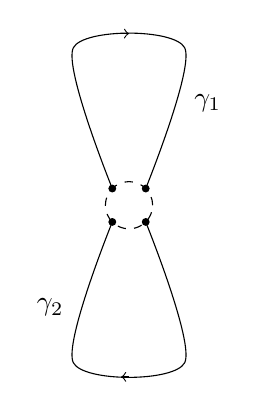
\begin{tikzpicture}
    \draw[dashed] (0,0) circle (.3);

    \fill (.3*.707, .3*.707) circle (.05)
          (.3*.707, -.3*.707) circle (.05)
          (-.3*.707, .3*.707) circle (.05)
          (-.3*.707, -.3*.707) circle (.05);
          %(0,2.18) circle (.05)
          %(0,-2.18) circle (.05);

    \draw[->] plot coordinates {(-.1,2.18) (0,2.18)};
    \draw[smooth] plot coordinates {(-.3*.707,.3*.707) (-.707, 2) (.707, 2) (.3*.707,.3*.707)};

    \draw[smooth] plot coordinates {(-.3*.707,-.3*.707) (-.707, -2) (.707, -2) (.3*.707, -.3*.707)};
    \draw[<-] plot coordinates {(-.1,-2.18) (0,-2.18)};

    \draw (1,1.3) circle (0) node {$\gamma_1$};
    \draw (-1,-1.3) circle (0) node {$\gamma_2$};
\end{tikzpicture}
    \caption{This draw relies on the graphical representation discussed in Section \ref{repr_su}. The dashed ball models the product representation carried by the Peter--Weyl state, each link represents the product factor and labels with $\alpha_i,\beta_i$ the linking nodes, on which the correspondent discretized gauge map is acting.}
\end{figure}
\,\newline
This shows that a functional in ${\Kk'}_\Gamma$ is not gauge--invariant, in general, but also, underscores that gauge--invariance $\Phi_*\psi=\psi$ is fulfilled for ${c'}^{\beta_1\beta_2}_{\alpha_1\alpha_2}=c^{\beta_1\beta_2}_{\alpha_1\alpha_2}$ {(i.e. $\varphi\cdot c=c$)} or, in the jargon of representations, coefficients $c$ must intertwine the spins ${j_i}$s. In other words, gauge--invariant states correspond to generators of isotropic subspaces of the product representation underlay by the Peter--Weyl basis.

By Theorem \ref{intert_isotrop} and by also arguing as in Example \ref{isotr_basis}, we infer that Figure 3.3 allows intertwiners among the representations of the two holonomies, corresponding to a $2$--dimensional isotropic subspace of the Peter--Weyl underlying representation, showing that multi--loop states are not independent
\begin{align*}
    \psi_I(U_\alpha,U_\beta)&=\rho^{\nicefrac{1}{2}}(U_\alpha)^A_B\,\rho^{\nicefrac{1}{2}}(U_\beta)^C_D\,\delta^B_A\delta^D_C\\
    &=\rho^{\nicefrac{1}{2}}(U_\alpha)^A_A\,\rho^{\nicefrac{1}{2}}(U_\beta)^C_C=\tr(U_\alpha)\tr(U_\beta)
\end{align*}
\begin{align*}
    \psi_{II}(U_\alpha,U_\beta)&=\rho^{\nicefrac{1}{2}}(U_\alpha)^A_B\,\rho^{\nicefrac{1}{2}}(U_\beta)^C_D\,\delta^D_A\delta^B_C\\
    &=\rho^{\nicefrac{1}{2}}(U_\alpha)^D_B\,\rho^{\nicefrac{1}{2}}(U_\beta)^B_D=\tr(U_\alpha\cdot U_\beta)
\end{align*}
\begin{align*}
    \psi_{III}(U_\alpha,U_\beta)&=\rho^{\nicefrac{1}{2}}(U_\alpha)^A_B\,\rho^{\nicefrac{1}{2}}(U_\beta)^C_D\,\epsilon^{BD}\epsilon_{AC}\\
    &=\rho^{\nicefrac{1}{2}}(U_\alpha)^A_B\,\rho^{\nicefrac{1}{2}}(\overline{U_\beta})^B_D=\tr(U_\alpha\cdot\overline{U_\beta})
\end{align*}
\,\newline
 Indeed, Example \ref{isotr_basis} here gives $\psi_{II}-\psi_I+\psi_{III}=0$, represented in the following

\begin{figure}[ht]
    \centering
    \includegraphics[scale=0.6]{images/multiloops.png}
\end{figure}
 
 \,\newline
 Farther, we got the following Proposition--Definition
\begin{defi}[Spin networks]
    For a lattice $\Gamma$, if a non--trivial spin representation $\rho^{(j)}$ on each link is given, together with an intertwiner on each node, then there exists a unique state in ${\Gg'}_\Gamma$ completely identified by the theory of irreducible representations of $\SU(2)$. We denote such state by $\ket{\Gamma;j_\Latt;i_N}$ and we call it a \emph{spin network}.
\end{defi}
It is worth observing here that
\begin{remark}[Spin networks basis]
    Choosing an independent set of intertwiners rules the ways of linking the different nodes and it also labels them. Thus, if one starts at a node and walks along a leaving line, it will be intertwined with a new node, forming a link which, soon or later, being the lattice finite, will close down to a \emph{(}possibly multi\emph{)} loop. Accordingly, spin networks are independent gauge--invariant multi--loop states, hence they form a \emph{(}still\emph{)} uncountable basis of $\Gg'$, though in ${\Gg'}_\Gamma$ they are countable.
\end{remark}


\subsubsection{\texorpdfstring{$\Diffeo(\Sigma)$}{a}--covariant states}
We now have to solve the diffeomorphism constraint equation for states, imposing $\Diffeo(\Sigma)$--invariance on spin networks. Unfortunately, one readily faces a hitch: by Peter--Weyl Theorem \ref{peter_weyl}, a diffeomorphism of the manifold maps a spin network in an orthogonal one, being affected even by slightly deformations of the $\Sigma$--embedded lattices they are associated with. Moreover, spin networks come with a precise orientation and ordering of the links, which are not left unchanged by the group $\Diffeo(\Sigma)$, in general (see Section 6.4 \cite{rov1}). For this reason, one has to deal with extended diffeomorphisms


\begin{defi}[Extended diffeomorphisms]
    A homeomorphism $\phi:\Sigma\to\Sigma$ of a smooth manifold such that it is a diffeomorphism on a finite number of points is said to be an \emph{extended diffeomorphism} and it writes $\phi\in\Diffeo_*(\Sigma)$.
\end{defi}
\,\newline
The action of $\Diffeo_*(\Sigma)$ can be now quotiented out from ${\Gg'}$ through the following argument: a given extended diffeo $\phi$ drags spin networks in spin networks, for which we write $\phi_*\ket{\Gamma;j_\Latt;i_\Latt}=\ket{\phi(\Gamma);j_\Latt;i_\Latt}$ and one can extend the left action to distributions $\Psi:\Gg\to\C$ in $\mathbb{G}$. For that, define the distribution
$$\begin{matrix}
    \phi^*\Psi:\Gg\to\C\\
    \quad\qquad\qquad\ket{S}\mapsto\Psi(\phi_*\ket{S})
\end{matrix}$$
on test--spin networks, from which one can ask $\Diffeo_*(\Sigma)$--invariance is addressed by states $\ket{S}\in\Gg$ satisfying the equation

\begin{equation}\label{diff_inv_states}
 (\phi^*\Psi)\ket{S}=\Psi\ket{S}   
\end{equation}
This yields a well--defined subspace of spin network functionals $\Psi\in\mathbb{D}\subseteq\mathbb{G}$ satisfying (\ref{diff_inv_states}), for any $\phi\in\Diffeo_*(\Sigma)$ and $\ket{S}\in\Gg$, and allows compatibility with the equivalence relation induced by $\ket{S}\sim\phi_*\ket{S}$ on $\Gg$, defining $\D:=\nicefrac{\Gg}{\sim}$. Moreover, it holds

\begin{teo}[Existence of $\Diffeo_*(\Sigma)$--invariant states]
    There exists a \emph{(}separable\emph{)} subspace $\D'$ of $\Gg'$ made of $\SU(2)$ and $\Diffeo_*(\Sigma)$ invariant kinematical states.
\end{teo}
\begin{proof}[Idea of the proof]
    Consider a gauge--invariant state on the form $\Psi_S\in\Gg$ and let $p(\Psi_S):\Gg\to\C$ be the linear map
    $$p(\Psi_S)\Psi_{S'}=\sum_{\Psi=\phi_*\Psi_S}\langle\Psi,\Psi_{S'}\rangle$$
    for $\phi\in\Diffeo_*(\Sigma)$. In order to prove continuity we claim the sum being finite. Let us expand $\Psi_S,\Psi_{S'}$ in the spin networks basis and take advantage of their graphical representations. Computing $\phi_*\ket{S}$ affects the sum in two possible ways: either the transformed graph is the same of $\ket{S'}$ or it is not. In the former, they must differ by a necessarily finite number of choice representations on each loop, while in the latter they have to be orthogonal states, hence there is no contribution to the sum. Furthermore, the state $p(\Psi_S)\in\mathbb{G}$ is $\Diffeo_*(\Sigma)$--invariant, since
    \begin{align*}
        \phi^*p(\Psi_S)\,\Psi_{S'}&=p(\Psi_S)\phi_*\Psi_{S'}=\sum_{\Psi={\phi'}_*\Psi_S}\langle\Psi,\phi_*\Psi_{S'}\rangle\\
        &=\sum_{\overline{\phi}_*\Psi=\overline{\phi}\circ{\phi'}_*\Psi_S}\langle\overline{\phi}_*\Psi,\Psi_{S'}\rangle=p(\Psi_S)\Psi_{S'}
    \end{align*}
    The above extends from spin networks to the whole $\Gg$ by linearity, yielding $p:\Gg\to\mathbb{D}\subseteq\mathbb{G}$ to be a projection to the quotient $\nicefrac{\Gg}{\sim}$ induced by $\ket{S}\sim\phi_*\ket{S}$. Once such a $p$ is well--defined, an inner product $(\cdot,\cdot):\mathbb{D}\times\mathbb{D}\to\C$ is well--defined by
\begin{equation}
    \bigg(p(\Psi_S),p(\Psi_{S'})\bigg):=p(\Psi_S)(\Psi_{S'})=\sum_{\phi\in\Diffeo_*(\Sigma)}\langle\phi_*\Psi_S,\Psi_{S'}\rangle
\end{equation}
and it induces the rigged Hilbert space $\D\subset{\D}'\subset\mathbb{D}$.
\end{proof}
We just got the following Proposition--Definition

\begin{defi}[Spin knots]
    A \emph{spin knot} is defined to be a basis for $\D'$, hence a $\Diffeo_*(\Sigma)$--invariant spin network, \emph{i.e.} it is a kinematical state satisfying both the gauge and the natural symmetries of Holst theory expressed in equation \emph{(\ref{constr_eqs_psi})}, at a quantum level.
\end{defi}

The whole above construction yields spin knots to be equivalence classes of spin networks, up to extended diffeomorphisms;\, it is not a subset of spin networks in $\Gg'$ with an additional property. In other words, we have to expect the space of spin networks to project onto the space of spin knots, not to be embedded into it\footnote{A final note on the separability of $\D'$. As a consequence of Theorem 3.1.7 and Definition 3.1.10, since the sum in (3.3) is finite, spin knots form a countable basis for $\D'$, which then turns out to be a separable Hilbert space of quantum states. Eventually, the non--separability of $\Gg'$ turns out to be just a gauge artifact---see Section 6.4.2 of \cite{rov1}.}. 

%\begin{remark}[Separability of $\D'$]
 %   As a consequence of \emph{Theorem 3.1.7} and \emph{Definition 3.1.10}, since the sum in \emph{(3.3)} is finite, spin knots form a countable basis for $\D'$, which then turns out to be a separable Hilbert space of quantum states. Eventually, the non--separability of $\Gg'$ turns out to be just a gauge artifact $($see \emph{Section 6.4.2} of \emph{\cite{rov1}}\emph{)}.
%\end{remark}

%As a final...
%$$\vdots$$
%$$\text{\textcolor{red}{Concludi sottolineando $\D'_\Gamma$ separabile e che a questo livello conta solo $\Gamma$ astratto}}$$
%$$\text{\textcolor{red}{aggiungendo che questo non è il vero $\mathcal{H}_{\text{phys}}$ which}}$$
%$$\text{\textcolor{red}{should contain spin foams, as mentioned in...}}$$
%$$\text{\textcolor{red}{vd anche "Reloading Hilbert spaces}}$$

\newpage
\subsection{Invariant operators among \texorpdfstring{$\mathcal{H}_\Gamma$}{a}}
Once a separable Hilbert space $\mathcal{H}_\Gamma$ is there for quantum invariant states, one proceeds to find out well--defined operators in $\Aut(\mathcal{H}_\Gamma)$, looking for the algebra of observables of the gravitational field. It has to be noticed that the operators which matter here would be the ones defined on spin knots or, at least, on spin networks, which then should be $\Diffeo_*(\Sigma)$--quotiented.\, By the way, two non--invariant operators, which will turn out to be related with gauge--connections, arise quite naturally.

We have already got a glimpse of how a Lie algebra element $\theta^i\tau_i\in\su(2)$ acts on a product state, by acting once at each link at a node. For instance, in a product representation $\rho^{j_1}\otimes\rho^{j_2}\otimes\rho^{j_3}$, being graphically represented as a trivalent node with $3$ links having spins $(j_1,j_2,j_3)$, if we consider $\tau_i$ acting on a Peter--Weyl state $\psi(U_1,U_2,U_3)={\rho^{j_1}(U_1)}^{\alpha_1}_{\beta_1}\,{\rho^{j_2}(U_2)}^{\alpha_2}_{\beta_2}\,{\rho^{j_3}(U_3)}^{\alpha_3}_{\beta_3}$, we are allowed to distribute it as
\begin{align*}
    \tau_i\bigg(\psi(U_1,U_2,U_3)\bigg)&=\tau_1\bigg({\rho^{j_1}(U_1)}^{\alpha_1}_{\beta_1}\bigg)\,{\rho^{j_2}(U_2)}^{\alpha_2}_{\beta_2}\,{\rho^{j_3}(U_3)}^{\alpha_3}_{\beta_3}+\\
    &\quad+{\rho^{j_1}(U_1)}^{\alpha_1}_{\beta_1}\,\tau_i\bigg({\rho^{j_2}(U_2)}^{\alpha_2}_{\beta_2}\bigg)\,{\rho^{j_3}(U_3)}^{\alpha_3}_{\beta_3}+\\
    &\quad+{\rho^{j_1}(U_1)}^{\alpha_1}_{\beta_1}\,{\rho^{j_2}(U_2)}^{\alpha_2}_{\beta_2}\,\tau_i\bigg({\rho^{j_3}(U_3)}^{\alpha_3}_{\beta_3}\bigg)
\end{align*}
Let us stress here that in each term the element $\tau_i$ acts on one link only, in the understood relevant representation $\T(\rho^{j_1}\otimes\rho^{j_2}\otimes\rho^{j_3})$. This suggests to define an operator ${L_{(n,\gamma)}}_i$ acting on one link $\gamma$ at a node $n$ by letting $\tau_i$ act on the factor corresponding to the link.

\begin{defi}[Lie operator]
    Let $\ket{\psi}\in\Kk'$ and $\theta^i\tau_i\in\su(2)$ such that $$\tau_i\ket{\psi}=\sum_{\gamma\in\Latt}{L_{(n,\gamma)}}_i\ket{\psi}$$
    A \emph{Lie operator} ${L_{(n,\gamma)}}_i$ is defined to be acting via the representation $\T\otimes_k\rho^{j_k}$ as$$\tau_i\bigg[\psi(U_1,\hdots,U_\Latt)\bigg]=\tau_i\bigg(\rho^{(j_1)}(U_1)^{\alpha_1}_{\beta_1}\bigg)\,\rho^{(j_2)}(U_2)^{\alpha_2}_{\beta_2}\hdots\rho^{(j_\Latt)}(U_\Latt)^{\alpha_\Latt}_{\beta_\Latt}\,+$$
    $$\qquad\qquad+\hdots+\rho^{(j_1)}(U_1)^{\alpha_1}_{\beta_1}\hdots\rho^{(j_{\Latt-1})}(U_{\Latt-1})^{\alpha_{\Latt-1}}_{\beta_{\Latt-1}}\tau_i\bigg(\rho^{(j_\Latt)}(U_\Latt)^{\alpha_\Latt}_{\beta_\Latt}\bigg)$$
    distributing Leibnitz--like, for any $(n,\gamma)\in\Gamma$.
\end{defi}
%Roughly speaking, a Lie operator ${L_{(n,\gamma)}}_i$ takes a Peter--Weyl basis element $\ket{\Gamma;j_\Latt}$ of a certain lattice, selects the links $\gamma\in\Latt$ one by one and attaches an element $\T\rho^{(j)}(\tau_i)^\alpha_\beta\ket{\Gamma;j;^\alpha,_\beta}$ to each one.\textcolor{red}{(?)} 

So far, Lie operators are nothing but a convenient way to write the action of operators which are polynomial in the Lie algebra $\su(2)$ in the product representations, using the product basis.

Let us define the subsets of $\Latt$ made by all the incoming and outgoing links $\Latt(n):=:i(n)\cup o(n)$, with respect to the node $n\in N$: then, if $\gamma\in i(n)$, the operator ${L(n,\gamma)}_i$ inserts a $\tau_i\in\su(2)$ (in the representation $\rho^j$ labelling the link) to the right of the factor corresponding to the link, while if $\gamma\in o(n)$ it insert a $-\tau_i\in\su(2)$ in the same way, but on the left.

\begin{prop}[Quantum closure condition]\label{quantum_closure}
    {Define for the Lie operator ${L_{(\nu,\gamma)}}_i:\Kk'\to\Kk'$ the following $C_\nu:=\sum_{\gamma\in\Latt(\nu)}{L_{(\nu,\gamma)}}_i$. Then $C_\nu\ket{S}=0$ \emph{iff} $\ket{S}\in\Gg'$}.
\end{prop}
\begin{proof}

We already saw in Proposition 3.3.1 that discretized gauges $\phi\in\mathscr{G}$ are given by a group element on the form $\exp(-\epsilon\,\theta^i\tau_i)\in\SU(2)$ at each node $n\in N$, hence they act on $\gamma\in i(n)$ by multiplication on the right and on $\gamma\in o(n)$ by inverse--multiplication on the left. Differentiating with respect to $\epsilon=0$ yields
$$\T\phi\ket{\psi}=\sum_{\gamma\in\Latt(n)}\theta^i{L_{(n,\gamma)}}_i\ket{\psi}$$
which clearly vanishes on invariant gauge--states $\ket{S}\in\Gg'$ since $\phi\ket{S}=\ket{S}$ implies $\T\phi\ket{S}=0$, being a derivation, provided that such a restriction is allowed.
\end{proof}
\,\newline
Despite this useful property, Lie operators do not restrict on spin networks, being $\tau_i$ not an intertwiner, in general, though some combination of them does. For instance, it can be checked that ${L^2_{(\nu,\gamma)}}:={L_{(\nu,\gamma)}}_i\delta^{ij}{L_{(\nu,\gamma)}}_j:\Gg'\to\Gg'$ is a well--defined operator. Indeed, it essentially inserts $\tau_i\delta^{ij}\tau_j$ at the nodes depending on whether $\gamma$ is incoming or outgoing: Remark \ref{Casimir} also implied $\tau_i\delta^{ik}\tau_k=\tau^2=j(j+1)\mathbb{1}$, for some spin representation $\T\rho^j$ of $\tau_i$,   which is clearly an intertwiner by Theorem \ref{shur}, providing spin networks to be eigenstates $L^2_{(\nu,\gamma)}\ket{S}=j(j+1)\ket{S}$. %$L_2_{(\nu,\gamma)}\ket{\Gamma;j_\Latt;i_N}=-j(j+1)\ket{\Gamma;j_\Latt;i_N}$.



\begin{defi}[Holonomy operators]
Recall parallel transport of a discrete connection $\Pp_\A[\gamma]\leftrightarrow\h(\A,\gamma)\in\SU(2)$ being represented by a special unitary matrix with entries ${\h(\A,\gamma)}^A_B\in\C$, as well as its spin representation $\rho^{(j)}(\h)^\alpha_\beta\in\C$. It is natural to define the operator $\h^{(j)}_\gamma:{\Kk'}\to{\Kk'}$ as acting multiplicative on cylindric functionals as
$$\h^{(j)}_\gamma\,^\alpha_\beta\cdot\psi_{\Gamma,f}(\h_1,\hdots,\h_\Latt):=\rho^{(j)}
(\h)^\alpha_\beta \,f(\h_1,\hdots,\h_\Latt)$$
It results to be the \emph{holonomy operator} of the connection $\h\in\SU(2)^\Latt$.
\end{defi}
\,\newline
On a Peter--Weyl basis it holds
$$\begin{matrix}
    \h_\gamma^{(j)}\,^\alpha_\beta:{\Kk'}_\Gamma\to{\Kk'}_{\Gamma\cup\gamma}\\
    \qquad\qquad\qquad\ket{\Gamma;j_\Latt,^{\alpha_\Latt},_{\beta_\Latt}}\mapsto\left|\Gamma\cup\gamma;j_\Latt,j,^{\alpha_\Latt,\alpha},_{\beta_\Latt,\beta}\right\rangle
\end{matrix}$$

\begin{remark}
    Holonomy operator is not gauge--invariant, since no intertwiners telling how to move among nodes are there, unless the link is a loop. Indeed, loops come with intertwiners and induces spin networks as gauge--invariant states, in which case $T_\gamma:=\h_\gamma^{(j)}:\Gg'\to\Gg'$, which stands as a trace operator, regarding a spin network as a superposition of loop states\footnote{Notice that such $T_\gamma$ resembles a \emph{creation operator} for LQG; indeed, if we let $\ket{\emptyset}\in\Gg'$ be the \emph{vacuum state} being the spin network with no nodes and no links, corresponding to the constant functional $1$ with no argument, we can produce any other spin networks by attaching links $\gamma$ to it, via holonomy operators $T_\gamma$.}.
\end{remark}

{Lie and holonomy operators are the building blocks of spacetime observables: they are operators representing discrete gauge transformations and connections and generate a sub--algebra of $\Aut(\Kk')$.} We refer to them as \emph{fundamental operators} and, since they are well--defined on Peter--Weyl states, hence in the whole $\Kk'$, we can compute their commutation relations (see \cite{LN8}), resulting as

\begin{equation}\label{commutator}
    \begin{split}
        \left[T_{\gamma},T_{\gamma'}\right]&=\mathbb{0}\\
        \left[{L_{(n,\gamma)}}_i,{L_{(n',\gamma')}}_j\right]&=-\delta_{nn'}\delta_{\gamma\gamma'}{\epsilon^k}_{ij}{L_{(n,\gamma)}}_k\\
        \left[{L_{(n,\gamma)}}_i,T_{\gamma'}\,^A_B\right]&=\begin{cases}
    -\delta_{nn'}(\tau_i)^A_CU^C_B&\text{if $\,\,\gamma\,\,$ outgoing}\\
    -\delta_{nn'}(\tau_i)^A_CU^C_B&\text{if $\,\,\gamma\,\,$ incoming}
\end{cases}
    \end{split}
\end{equation}
\,\newline
They hence generate an algebra of operators still on kinematic states, which are not yet invariant, hence they do not close to an algebra of operators in $\Gg',\D'$. First quantisation suggests to look for a sub--algebra of operator which does take in spin networks first and spin knots then, that thereupon can be regarded as observables of space--geometry (not yet spacetime, for which we would need spin--foams in $\Pp'$).\, Notice that, aiming to restrict operators on spin knots, for a given $\phi\in\Diffeo_*(\Sigma)$ we can define
$$\begin{matrix}
    \phi^*T_\gamma:\Gg'\to\Gg'\\
    \qquad\qquad\qquad\ket{S}\mapsto T_{\phi_*\gamma}(\phi_*\ket{S})
\end{matrix}$$
which is compatible to the quotient in Theorem 3.1.7. Moreover, Lie operators do depend only on \emph{adjacency}, a trait which is not affected by extended diffeomorphisms; hence, they also are $\Diffeo_*(\Sigma)$--invariant.\\

Looking forward the construction of the $\Aut(\Kk')$--sub algebra made of observables of the space--geometry, we choose to conclude this section by recovering some other important geometric operator, at least from a historical point of view.



\subsubsection{Link and area operators}
For fixed $\gamma,\nu\in\Gamma$ one has the following gauge--invariant (so--called link) operator
\begin{equation}\label{area_op}
    {E_\gamma}^2=E_{(\nu,\gamma)}\cdot E_{(\nu,\gamma)}:=(\hslash\boldsymbol{\kappa}\boldsymbol{\gamma})^2\bigg|{L_{(\nu,\gamma)}}_i\delta^{ij}{L_{(\nu,\gamma)}}_j\bigg|=\left(\hslash\boldsymbol{\kappa}\boldsymbol{\gamma}L_{(\nu,\gamma)}\right)^2
\end{equation}
which inserts $(\hslash\boldsymbol{\kappa}\boldsymbol{\gamma})^2\tau_i\delta^{ij}\tau_j$ between the node $\nu\in N$ and the link $\gamma\in\Latt(\nu)$. In the spin representation $\rho^j$, Remark \ref{Casimir} yields ${E_\gamma}^2=\hslash\boldsymbol{\kappa}\boldsymbol{\gamma})^2j(j+1)\mathbb{1}$ and also allows spin networks as eigenstates. 

The above \emph{link operator} has hence a discrete spectrum $\bigg\{(\hslash\boldsymbol{\kappa}\boldsymbol{\gamma})^2j(j+1)\bigg\}_{j\in\frac{1}{2}\N}$ made of positive eigenvalues, and allows to define the so--called \emph{area operator} as $A_\gamma:=\sqrt{{E_\gamma}^2}$, which hence satisfies
\begin{equation}\label{area_spec}
    A_\gamma\ket{S}=\hslash\boldsymbol{\kappa}\boldsymbol{\gamma}\sqrt{j(j+1)}\ket{S}
\end{equation}
By noticing that the constant $\hslash\boldsymbol{\kappa}\boldsymbol{\gamma}$ has the dimension of an area, the physical interpretation here would come clear: each link $\gamma$ of a spin network carries a quantum of area of the space which, if measured, can only assume discretized values of the form 
$$0\qquad\hslash\boldsymbol{\kappa}\boldsymbol{\gamma}\frac{\sqrt{3}}{2}\qquad\hslash\boldsymbol{\kappa}\boldsymbol{\gamma}\sqrt{2}\qquad\hdots\qquad\hslash\boldsymbol{\kappa}\boldsymbol{\gamma}\sqrt{j(j+1)}\qquad\hdots$$
It has to be noticed that such a concept of quantum area is strictly related to a spin network: this is natural still, because invariant states define the gravitational field---which is identified with space(time) geometry---at a quantum level, and no any quantum geometrical aspect of the spacetime should be detected unless with respect to the quantum physical states.

Let us extend the above to the area of a surface: let $\Omega$ be a closed and orientable $2$--manifold and consider a spin network $\ket{S}=\ket{\Gamma;j_\Latt;i_N}$, then either $\Gamma\cap\Omega=\emptyset$ or $\Gamma\cap\Omega\neq\emptyset$ is finite (being the lattice a finite collection of links and nodes in $(\Latt,N)$). If the intersection is empty, there is no area to compute with respect to $\ket{S}$; if not, let $k_i\in\Gamma\cap\Omega$ and consider so an open patch $U_i\subseteq\Omega$ which intersects one and only the point $k_i$. A homotopical--argument shows that there is no loss of generality in assuming the links of $\Gamma$ to be transverse to the surface $\Omega$, intersecting zero times or once with $k_i$ as an endpoint, in each open patch $U_i$. This way, for such a $\gamma_i\in\Latt(k_i)$ it holds $A(U_i)\ket{S}=\hslash\boldsymbol{\kappa}\boldsymbol{\gamma}\sqrt{j_i(j_i+1)}\ket{S}$ and
$$A(\Omega)\ket{S}:=\sum_{k_i\in\Gamma\cap\Omega}A(U_i)\ket{S}=\sum_{k_i\in\Gamma\cap\Omega}\hslash\boldsymbol{\kappa}\boldsymbol{\gamma}\sqrt{j_i(j_i+1)}\ket{S}$$
is a well--defined operator for the quantum area of $\Omega$, assuming $A(U_0)\ket{S}=0$ for an open patch $U_0$ not intersecting $\Gamma$, in the case $\Omega\cap\Sigma=\emptyset$.

%Since the state is eventually a superposition of spin knots, just because it has to be gauge and $\Diffeo_*(\Sigma)$--covariant, it makes no sense to define the area of a “fixed” surface $\Omega$ with respect to a spin knot (i.e. with respect to an equivalence class of spin networks). Different representative spin networks of the same spin knots would get different areas, i.e. the area would not be compatible with the quotient with respect to $\Diffeo_*(\Sigma)$.
%The only quantity which is well defined is the area of the dragged surface $\phi(\Omega)$ with respect to the dragged spin network $\phi_*\ket{S}$, which is in fact compatible with the quotient, hence it defines a quantity which belongs to the spin knots.

%\subsubsection{Volume operator}

%meglio metterlo dopo perchè ha a che fare coi tetraedri e si capisce meglio lì
{As a final summarizing remark
\begin{remark}[Section 6.6.2 \cite{rov1}]
    At this stage, it can be noticed that the smallest non--vanishing eigenvalue of the area operator $A_\gamma\in\Aut(\Gg')$, by taking the Holst parameter equal to $1$, can be computed approximately as $4\sqrt{3}\pi\hslash Gc^{-3}\approx10^{-66}\,\text{\normalfont{cm}}^2$, corresponding to an elementary quantum of area, being of the same order of the Planck area. It is a quantum of area carried by a link in the fundamental representation $j=\frac{1}{2}$, within a spin network.
\end{remark}
}
{Such an intrinsic discreteness of physical space at the Planck length has long been expected in quantum gravity and it has been reached here as a direct consequence of the theory.}


\subsubsection{Conjugate momentum operator}

%Necessario per avere la quantizzazione delle variabili canoniche $\A,\E$
Recall (\ref{conj_momenta_holst}) for the ABI--conjugated momentum being $p^a_i=\frac{1}{\boldsymbol{\kappa\gamma}}\E^a_i$, whose quantisation should be represented by the densitized triad being promoted to an operator of the form
$$\E^a_i=-i\hslash\boldsymbol{\kappa\gamma}\frac{\delta}{\delta\A^i_a(k)}:\Kk'\to\Kk'$$
which acts on a Peter--Weyl state $\ket{\Gamma;j_\Latt}$, said $\gamma\in\Latt$, as follow
\begin{align*}
    \E^a_i\rho^{(j)}(\h_\gamma)&=-i\hslash\boldsymbol{\kappa\gamma}\frac{\delta\rho^{(j)}(\h_\gamma)}{\delta\A^i_a(k)}\\
    &=-i\hslash\boldsymbol{\kappa\gamma}\rho^{{(j)}}(\h_{\gamma_1})\T\rho^{(j)}(\tau_i)\rho^{(j)}(\h_{\gamma_2})\int_\gamma{\dot{k}^a(s)\delta^3(k-k(s))}\d s
\end{align*}
since $p^i_a\,\rho^{(j)}(\h_\gamma)$ vanishes on $k\in\Sigma\setminus\gamma(0,1)$, while if $k\in\gamma$ then a $2$--valence node can be put at $k$, splitting $\gamma=\gamma_1*\gamma_2$ and adding an element $\pm\tau_i\in\su(2)$ at the node, which is exactly what the above expression does\footnote{We refer to Appendix A of \cite{LN5} for explicit computation of the variation of the holonomy given by $\h_\gamma\in\SU(2)$ with respect to the connection.}. This way, if $\Omega\hookrightarrow\Sigma$ is an oriented surface, one defines
$$\E^a_i(\Omega)\rho^{(j)}(\h_\gamma):=\int_\Omega\E^a_i\rho^{(j)}(\h_\gamma) u_\alpha\d\sigma$$
said $\d\sigma$ the local volume element induced by coordinates $\sigma^i$ on $\Omega$ and $u_\alpha$ the canonical covector of $\Omega\subseteq\Sigma$. %Assume the link $\gamma$ to be transverse to $\Omega$, having only one point of intersection at $k\in\Omega\cap\Gamma(0,1)$



%\subsubsection{Some others invariants}
%It needs "Reloading Hilbert spaces"


\newpage
\section{Towards the quantum geometry of spacetime}
In this section we will work out a fundamental class of invariant operators in $\Gg'$ (hence in $\D'$) by leaning on a correspondence between classical and quantum discrete geometries.\, As one may have already got a glimpse in the previous, LQG proposes a model for a generally covariant quantum field theory, turning out to fit better with a first quantisation--like procedure instead of being treated as a true QFT, subjected to second quantisation (CFR Section \ref{first_quantisation}). 

Once one detects the classical invariant states to be discrete connections $\h\in\SU(2)^\Latt$ up to gauge transformations, the natural choice for the quantum space results in its cotangent bundle. Therefore, recovering the quantisation of the classical Poisson algebra of the cotangent bundle over $\SU(2)$ turns out to be a key step.\\ %Spin networks and spin knots have been defined to eventually provide a quantisation of spatial geometries on S which is covariant (with respect to the gauge group and $\Diffeo_*(\Sigma)$), background free, in some sense non-perturbative. It is still not a quantisation of gravity, which would be a quantisation of spacetime geometries (or implementing the Hamiltonian constraint), even though it provides many tools for it. In view of the discussion of Cauchy bubbles, spin networks are a theory at the bubble boundary for quantum gravity; in other words they are pre--quantum states for gravity.


%\begin{remark}[Physical interpretation of spin networks]
    %The essential property of the volume operator is that it takes contribution only from the nodes of a spin network $\ket{S}$: the volume of a region appears as a sum with as many terms as the nodes of $S$ inside the region. Therefore, to each node of a spin network can be given the interpretation of representing a quantum of volume.
%\end{remark}
%$$\text{continua in 6.7 \cite{rov1}}$$

 %\subsubsection{Poisson algebra of \texorpdfstring{$T^*\SU(2)^\Latt$}{a}}

By summarizing, our classical theory had canonical variables $(\A^i_a,\E^a_i)$ which correspond to the holonomy and momentum operator in the quantisation that we have developed so far. Their commutation relations are completely understood by (\ref{commutator}), which, for later convenience, can be read in each $\SU(2)$ component as
\begin{equation}\label{commutator_simple}
    \begin{cases}
        [\h,\h]=\mathbb{0}\\
        [L_i,L_j]={\epsilon^k}_{ij}L_k\\
        [L_i,\h]=-\h\tau_i
    \end{cases}
\end{equation}
where $\h,L_i$ stand for the holonomy operator related with $\A$ and the Lie operator related with $\E$, respectively. We want now to provide the reader with an evidence that such a Lie algebra realizes as the quantisation of the Poisson bracket induced by the symplectic structure of $T^*\SU(2)^\Latt$, being nothing but $\Latt$ copies of $T^*\SU(2)\cong\SU(2)\times\su(2)^*$\footnote{A Lie group $\G$ is necessarily parallelizable: once a basis $\{\T_i\}$ of $\mathfrak{g}$ is fixed, left--invariant frame and coframe are always there \emph{global}, induced by $\rho_i=R^a_i\frac{\der}{\der\g^a}\in\mathfrak{g}$. Moreover, there are no restrictions on the existence of a dual basis $\theta^i_a\d\g^a$ to $\rho_i$, which induces a symplectic structure of cojugated coordinates $(\g^a,\theta_a)\in T^*\G$ and Poisson bracket $\{f,g\}=\frac{\der f}{\der\theta_a}\frac{\der g}{\der{\tiny}\g^a}-\frac{\der f}{\der\tiny\g^a}\frac{\der g}{\der\theta_a}$, which closes $T^*T^*\G$ to a Lie algebra.}. 

\begin{teo}
    Holonomy and Lie operators satisfying \emph{(\ref{commutator})} are in place as a quantisation of the Poisson algebra of $T^*\SU(2)^\Latt$.
\end{teo}
\begin{proof}[Idea of the proof]
    We consider a proof for only one of the $\SU(2)$ copies. Let $(U,\ell_i\theta^i)$ be a pair of coordinates on $T^*\SU(2)$, then, once the basis $\{\tau_i\}_{i=1,2,3}$ is fixed on $\su(2)$, one gets 
$$\lambda_i:=-U^C_A\,{\tau_i}^A_B\frac{\der}{\der U^C_B}\qquad\qquad\theta^i:=2\delta^{ik}{\tau_k}^D_E\overline{U}^E_F\,\d U^F_D$$
as global left--invariant frame fields, where we are looking at $\SU(2)$ as a manifold embedded in $\GL(2,\C)$ through $U\mapsto U^A_B$ as a special unitary matrix (i.e. $\overline{U}^A_BU^B_C=\delta^A_C$ and $\frac{1}{2}\epsilon_{AC}U^A_BU^C_D\epsilon^{BD}=1$). This way, the above span basis dual to each other as
\begin{align*}
    \theta^i(\lambda_j)&=-2\delta^{ik}{\tau_k}^D_E{\tau_j}^A_B\overline{U}^E_FU^C_A\delta^F_C\delta^B_D\overbrace{=}^{\overline{U}^E_C=\overline{U}^E_F\delta^F_C}-2\delta^{ik}{\tau_k}^D_E{\tau_j}^A_B\delta^E_A\delta^B_D\\
    &=-2\delta^{ik}{\tau_k}^D_A{\tau_j}^A_D=-2\delta^{ik}\tr(\tau_k\cdot\tau_k)=\frac{1}{2}\tr(\delta^i_j\mathbb{1}-2{\epsilon_j}^{il}\tau_l)\\
    &=\delta^i_j
\end{align*}
and the constraints imposed by the embedding
%Moreover it can be checked $[\lambda_i,\lambda_j]=\epsilon_{ij}^k\lambda_k$, resembling angular momenta of the group, 
 can be differentiated and so lifted to the cotangent bundle, giving conjugated momenta to $U^A_B$ in the form $p^A_C=2\ell_i\delta^{ik}{\tau_k}^A_B\overline{U}^B_C$ in $\GL(2,\C)$. On the other hand, we know the Poisson bracket satisfies $\{U^A_B,p_C^D\}=\delta^A_C\delta_B^D$ by duality, thus, by inverting 
 $$p^A_CU^C_B{\tau_j}^B_A=2\ell_i\delta^{ij}\tr(\tau_k\cdot\tau_j)\quad\Rightarrow\quad \ell_i=-p^A_CU^C_B{\tau_i}^B_A$$
one computes Poisson bracket on $T^*\SU(2)$ as
$$\begin{cases}
    \{U^A_B,U^C_D\}=\mathbb{0}\\
    
    \{\ell_i,\ell_j\}={\epsilon^k}_{ij}\ell_k\\
    \{U^A_B,\ell_i\}=-U^A_C{\tau_i}^C_B
\end{cases}$$
which corresponds to (\ref{commutator_simple}) and the proof is accomplished.
\end{proof}
{Accordingly, \emph{kinematical }LQG (still in $\Kk'$) resembles a canonical quantisation of a classical mechanics--like theory on the configuration space $\SU(2)^\Latt$ working as a model for classical geometry of space. Indeed, geometry has the aim to describe the (classical) physical laws of space since ever and LQG suggests to interpret the quantum texture of space as spin networks. The most interesting case we handled is the one yielded by 4--valence nodes, which corresponds to \emph{quantum tetrahedra}.}

%This is the perfect time to present, as an interlude, the discrete geometry of a classical tetrahedron.


\subsection{Classical geometry of tedrahedra}

%Spin networks and spin foams.

%\subsection{Matter coupling}
%Main references \cite{rov2}
Tetreahedra are $3$--simplexes completely identified by four vertices $(x_0,x_1,x_2,x_3)\in\Sigma$, hence by $12$ scalars. The \emph{geometry} of a tedrahedron is meant to be the metric properties up to isometries. Its classical geometry is determined so by $12-6=6$ degrees of freedom, having quotiented--out the $3+3$ rotations and translations of $\GL(3)$. We want to construct a Lie algebra made of geometric observables for the tedrahedron, that we expect to contain its volume, the areas of its four faces and the lengths of its six sides, as well as its dihedral angles and, in general, all geometric quantities.

A tetrahedron has $4$ oriented \emph{faces} being $2$--simplexes, with boundaries made of oriented $1$--simplexes; it also counts $6$ \emph{edges} (or \emph{sides}).\, Let us conventionally set $x_0$ to identify the tip of the pyramid and $x_1,x_2,x_3$ to be vertices of the base triangle, then we set for the sides $\s_{\alpha\beta}$ and faces $\ff_\alpha$
$$\begin{matrix}
    \s_{01}:=[x_0,x_1] & \s_{02}:=[x_0,x_2] & \s_{03}:=[x_0,x_3]\\
    \s_{12}:=[x_1,x_2] & \s_{13}:=[x_1,x_3] & \s_{23}:=[x_2,x_3]
\end{matrix}$$
$$\begin{matrix}
    \ff_0=[x_1,x_2,x_3] & \ff_1=-[x_0,x_2,x_3] &\ff_2=[x_0,x_1,x_3] &\ff_3=-[x_0,x_1,x_2]
\end{matrix}$$
We have two somehow dual representation of the tedrahedron, capturing its intrinsic geometry

\begin{itemize}
    \item (Sides representation)\,\,By fixing the origin at the tip $x_0$, the six edges are parametrized by their $18$ components, but they are also constrained by $\s_{ij}=\s_{0j}-\s_{0i}$. Accordingly, only the three vectors $\s_{0i}=:v_i$ are independent and generate the others $\s_{ij}$, thus they give $9$ independent parameters up to $3$ rotations, hence $6$ degrees of freedom to parametrize the invariant geometric quantities.

    \item  (Faces representation)\,\, For each faces $\ff_\alpha$, the four normal vectors are in place, defined as---recall in $\R^3$ the cross product satisfying  $v\wedge w=\frac{1}{2}v\times w$ 
    $$\begin{matrix}
        \l_0:=\frac{1}{2}\s_{12}\times\s_{13} & \l_1:=-\frac{1}{2}\s_{02}\times\s_{03} & \l_2:=\frac{1}{2}\s_{01}\times\s_{03} & \l_3:=-\frac{1}{2}\s_{01}\times\s_{02} 
    \end{matrix}$$
    Each $\l_\alpha$ accounts for the areas of $\ff_\alpha$ in magnitude, by definition, and the so--called \emph{classical closure condition}\footnote{CFR Proposition \ref{quantum_closure}.} $\l_0+\l_1+\l_2+\l_3=0$ holds true. Hence, only three of the four normals are independent and again there are $6$ parameters identifying the intrinsic geometry of a tedrahedron. 
\end{itemize}
Moreover, the two above representations of the discrete geometry of classical tedrahedra turn out to be equivalent: indeed, one sees that $v_i$ are parallel to $\frac{1}{2}{\epsilon_i}^{jk}\l_j\times\l_k$\footnote{Notice we could argue equivalently that $v_i\times v_j={\epsilon_{ij}}^k\l_k=:\l_{ij}$} and one proves (see \cite{LN9}) it holds---for $\omega^{-1}:=\sqrt{\l_1\cdot\l_2\times\l_3}$
$$\begin{matrix}
    v_1=\pm\omega\,\l_2\times\l_3 & v_2=\pm\omega\,\l_3\times\l_1 & v_3=\pm\omega\,\l_1\times\l_2
\end{matrix}$$

Accordingly, we can regard classical discrete geometries of a tetrahedron as points in the homogeneous space $\Geo:=\nicefrac{\GL(3)}{\SO(3)}$,
which is $6$--dimensional as a manifold---said, locally homeomorphic to $\R^6$. This way, the \emph{sides} and the \emph{faces} representations turn out to just represent two different local homeomorphisms among $\Geo$ and $\R^6$ through the correspondence given by points of $\Geo$ and $(v_i,v_j),(\l_i,\l_j)\in\R^6$ respectively.

Looking for a Poisson algebra representing the geometric observables of classical tedrahedra, we must turn our gaze towards function(al)s in $\Geo\to\R$, meaning scalar functions of $\GL(3)$ which are invariant under the action of $\SO(3)$. Else, we can hope to find out a set of \emph{six} fundamental geometric invariant quantities that may generate all the other geometric observables as their functions. 

For that, a suitable choice of such invariant functionals comes from the \emph{dihedral angles} $\theta_{\alpha\beta}:=\frac{\l_\alpha\cdot\l_\beta}{|\l_\alpha||\l_\beta|}$, which define the geometric invariants $\d_{\alpha\beta}:=\l_\alpha\cdot\l_\beta$\footnote{This choice of fundamental geometric invariants for the tetrahedron is clearly not unique. We are just fixing a set of operators that we expect to generate all the other geometric quantities as functions of them, by also aiming them to form an algebra. The intrinsic notion will be the invariant sub--algebra of fundamental geometric quantites they will define.}. A priori, a dihedral angle is described by $10$ parameters, being symmetric in $\alpha,\beta=0,\hdots,3$. 

It is easy to see the following relation hold true
$$\d_{00}=\sum_{\substack{i,j=1\\ i\neq j}}^3\d_{jj}+2\d_{ij}=\d_{00}(\d_{ij})\qquad\d_{0i}=-\sum_{j=1}^3\d_{ij}=\d_{0i}(\d_{ij})$$ 
implying that only the six $\d_{ij}$ are actually linear independent. Since, in the face representation, it holds $\left\{\l_i,\l_j\right\}={\epsilon^k}_{ij}\l_k$ for the normals, Leibnitz rule easily implies
\begin{align*}
    \left\{\d_{ij},\l_k\right\}&=\left\{\l_i\cdot\l_j,\l_k\right\}=\l_i\times\left\{\l_j,\l_k\right\}+\left\{\l_i,\l_k\right\}\times\l_j\\
    &={\epsilon_{jk}}^l\l_i\times\l_l+{\epsilon_{ik}}^l\l_l\times\l_j
\end{align*}
{which vanishes for $j=k$ and $i=k$ or $j\neq k$ and $i\neq k$, otherwise 
$$\left\{\d_{ij},\l_i\right\}={\epsilon_{ji}}^l\l_i\times\l_l\neq0$$}
This way, an analogous computation shows---for any $i,j,k\in\{1,2,3\}$
\begin{equation}\label{classical_geom_obs}
\begin{split}
    \left\{\d_{ij},\d_{jk}\right\}&=\l_i\times\l_j\cdot\l_k=:\d\\
    %\{\d_{ij},\d_{ii}\}&=0=\{\d_{ij},\d_{kk}\}\\
    \{\d,\d_{ij}\}&=\d_{jk}\d_{ii}-\d_{ik}\d_{jj}
\end{split}
\end{equation}
{which closes a Poisson algebra generated by $6$ independent (combination of) dihedral angles $\d_{ij}$, such that all the other geometric quantities of the tetrahedron depend on.} For that, it can be shown an important result
\,\newline
\begin{teo}[On geometric observables]\label{T^*Geo}
    A function $F:\GL^+(3)\to\R$ is $\SO(3)$--invariant if and only if it depends on the dihedral angles, \emph{i.e.} $F=F(\d_{ij})$.
\end{teo}
\begin{proof}
    It relies on a Utiyama--like argument (see Section \ref{utiyama} and also \cite{LN9}).
\end{proof}
Therefore, we have selected six geometric invariants $\d_{ij}$ that functionally generate an algebra of what can be regarded in this theory as geometric observables, endowed with a Poisson structure.
%geometric observables have been completely characterized as invariant functionals in $T^*\Geo$, being parametrized by the invariant coordinates $\d_{ij}$, and they are there with a Poisson algebra structure. 
This is not surprising from a geometrical point of view, but so is from a physical one, since there is not a real dynamics on $\Geo$, being its points discrete geometries.

Anyway, \emph{lengths} of sides are clearly functions of the $\d_{ij}$s, while for \emph{areas} of faces $\ff_\alpha$ it holds by construction $A_\alpha={(\d_{\alpha\alpha})}^{\frac{1}{2}}$ and for the \emph{volume} of the whole tetrahedron it holds by definition\footnote{Recall the triple product accounts for the signed volume $\epsilon^{abc}V=\mathbf{a}\cdot\mathbf{b}\times\mathbf{c}.$}
\begin{align*}
    v&:=\frac{1}{6}v_1\cdot v_2\times v_3=\frac{\sqrt{2}}{3}\left|\l_1\cdot\l_2\times\l_3\right|^{\frac{1}{2}}=\frac{\sqrt{2}}{3}|\d|^{\frac{1}{2}}
\end{align*}
For later convenience we leave here other useful characterisation
$$\l_1\cdot\l_2\times\l_3=-\frac{1}{2}\left\{\l_1\cdot\l_3,|\l_1+\l_2|^2\right\}=\d$$
where
$$\left|\l_1+\l_2\right|^2=\d_{11}+\d_{22}+2\d_{12}$$
which yields the following fundamental
\begin{equation}\label{volume}
    v^2=\frac{1}{9}\bigg|\left\{\l_1\cdot\l_3,|\l_1+\l_2|^2\right\}\bigg|
\end{equation}


A tedrahedron has so $4$ areas, $1$ volume, $6$ lengths and $6$ dihedral angles and all of them are geometric quantities though not independent, having classical discrete geometries $6$ degrees of freedom. This allows us to arbitrarily choose $6$ independent geometric quantities, among the so--called \emph{geometric algebra} that we proved being generated by $\d_{ij}$, to represent all the others as functionally dependent, in the flavour of Theorem \ref{T^*Geo}.

The key point here is that the discrete geometric observables for the tetrahedron that we have just described form not only a Lie algebra, yet a Poisson algebra, carrying so a symplectic structure.\, Moreover, they encode the $\SU(2)$--gauge covariance that we want to impose on our kinematical states still in $\Kk'$ to get operators in $\Gg'$, then in $\D'$. 

This is the very nice trait that makes physical theories so interesting and well--fitted to quantisation, and unravels a hope to reach a fundamental description of the spacetime texture as made of quantum fuzzy tetrahedra, in correspondence of $4$--valence spin networks.


\newpage
\subsection{Quantum geometry of LQG}\label{QuantumGeoTetrahedra_section}

LQG started as a second--quantisation of the ABI field theory, whose kinematical states were $\Psi(\A)\in L_2(\SU(2)^\Latt)$, and ended up to correspond to a first--quantisation of the Poisson algebra on $T^*\SU(2)^\Latt$. Farther, we are providing invariant LQG with the feature to be the quantisation of the discrete geometry of tetrahedra. For the sake of simplicity, set $j:=(n,\gamma_j)\in\Gamma$ labelling the links at the $4$--valence node $n$ and resume (\ref{commutator}) as
$$\left[{(L_i)}_a,{(L_j)}_b\right]=-\delta_{ij}{\epsilon_{ab}}^c{(L_i)}_c$$
By promoting classical dihedral angles $\d_{ij}$ to operators as $\Dd_{ij}:={(L_i)_a}\delta^{ab}{(L_j)_b}$, as yet in $\Kk'$, in analogy to the classical case, Leibnitz rule yields
\begin{align*}
    \left[\Dd_{ij},{(L_k)}_c\right]&=\delta^{ab}\left[{(L_i)}_a{(L_j)}_b,{(L_k)}_c\right]\\
    &=\delta^{ab}{(L_i)}_a\left[{(L_j)}_b,{(L_k)}_c\right]+\delta^{ab}\left[{(L_i)}_a,{(L_k)}_c\right]{(L_i)}_a\\
    &=-\delta^{ab}\delta_{jk}{(L_i)}_a{(L_j)}_d{\epsilon^d}_{bc}-\delta^{ab}\delta_{ik}{(L_i)}_d{(L_i)}_a{\epsilon^d}_{ac}
\end{align*}
{which is non--vanishing for $i\neq j$ and $k\in\{i,j\}$, resulting}
$$\left[\Dd_{ij},(L_i)_a\right]=\epsilon^{abc}{(L_i)}_b{(L_j)}_c=:\left(L_i\times L_j\right)^a$$
still implying---for each $i,j,k\in\{1,2,3\}$

\begin{equation}\label{commutation_dihedral_ops}
    \begin{split}
    \bigg[\Dd_{ij},\Dd_{jk}\bigg]&=L_i\times L_j\cdot L_k=:\Dd\\
    \bigg[\Dd,\Dd_{ij}\bigg]&=\Dd_{jk}\Dd_{ii}-\Dd_{ik}\Dd_{jj}\\
    &0\quad\text{otherwise}
\end{split}
\end{equation}
%{Hence, we got all the commutation relation among the dihedral operators, being $[\Dd_{0i},\Dd_{jk}]=[\Dd_{00},\Dd_{0i}]=[\Dd_{00},\Dd_{ij}]=0$ and $[\Dd_{ij},\Dd_{jk}]\neq0$}.\,
Moreover, we can also define the volume squared operator by promoting (\ref{volume}) to 
\begin{equation}\label{volume_op}
    V^2:=\frac{i\hslash}{9}\Biggl|\bigg[\Dd_{13},\Dd_{11}+\Dd_{22}+2\Dd_{12}\bigg]\Biggl|=\frac{2i\hslash}{9}\Biggl|\bigg[\Dd_{13},\Dd_{12}\bigg]\Biggl|:\Kk'\to\Kk'
\end{equation}
Farther, the quantum closure condition in this framework gives a characterisation of operators that restrict to $\Gg'$, in according to the following

\begin{teo}\label{op_gauge_invar}
    Consider an operator $\mathcal{O}:\Kk'\to\Kk'$ which satisfies $[\mathcal{O},C_\nu]=0$. Then actually $\mathcal{O}:\Gg'\to\Gg'$ is a gauge--invariant operator.
\end{teo}
\begin{proof}
    Consider a spin network state $\ket{S}\in\Gg'$, then by hypothesis 
    \begin{align*}
        0&=[\mathcal{O},C_\nu]\ket{S}=\cancel{\mathcal{O}C_\nu\ket{S}}-C_\nu\mathcal{O}\ket{S}
    \end{align*}
    $$\Leftrightarrow$$
    $$\mathcal{O}\ket{S}=0$$
    i.e. if and only $\mathcal{O}\in\Aut(\Gg')$, by Proposition \ref{quantum_closure}.
\end{proof}
\,\newline
{This gives a characterisation of geometric operators as being gauge--invariant, i.e. they represent physical observables in $\Aut(\Gg')$.}
{
\begin{cor}
    The dihedral angles $\Dd_{\alpha\beta}$, as well as the squared volume $V^2$, are invariant operators in $\Aut(\Gg')$.
\end{cor}}
{\begin{proof}
It is just a matter of computing commutators $[\Dd_{00},C_\nu],[\Dd_{0i},C_\nu],[\Dd_{ij},C_\nu],[V^2,C_\nu]$. Recall that we are in the framework of a $4$--valence node $\nu\in N$ where each link $\gamma_j\in\Latt(\nu)$ is labelled by an index $j$ which runs in $\{0,1,2,3\}$ and we set $j:=(n,\gamma_j)\in(N,\Latt)=\Gamma$ , with an abuse of notation. The operator $C_\nu=L_0+L_1+L_2+L_3$ combined with the quantum closure condition (see Proposition \ref{quantum_closure}) yields
    \begin{align*}
    \left[\Dd_{00},C_\nu\right]&=\sum_{i\neq j}\bigg[\Dd_{jj},L_0+L_1+L_2+L_3\bigg]+2\bigg[\Dd_{ij},L_0+L_1+L_2+L_3\bigg]=0\\
    [\Dd_{0i},C_\nu]&=-\sum_j\bigg[\Dd_{ij},L_0+L_1+L_2+L_3\bigg]=0\\
    [\Dd_{ij},C_\nu]&=[\Dd_{ij},L_i]+[\Dd_{ij},L_j]=L_i\times L_j-L_i\times L_j=0\\
    \left[V^2,C_\nu\right]&=\frac{2i\hslash}{9}\bigg[[\Dd_{13},\Dd_{12}],C_\nu\bigg]=-\frac{2i\hslash}{9}\Biggl(\bigg[[C_\nu,\Dd_{13}],\Dd_{12}\bigg]+\bigg[[\Dd_{12},C_\nu],\Dd_{13}\bigg]\Biggl)=0
    \end{align*}
    and Theorem 3.2.3 concludes.
\end{proof}
}
Up to now, we have pointed out an algebra of $6$ independent invariant---so--called \emph{geometric}---\emph{operators} $\Dd_{ij}$, which generate all the other geometric observables of a quantum tetrahedron, such as the squared volume $V^2$, the squared areas $\Dd_{00}$, $\Dd_{11}$, $\Dd_{22}$, $\Dd_{33}$, or $\Dd$, being polynomials in the $\Dd_{ij}$\footnote{{In other words, the algebra of geometric observables corresponds to the universal enveloping algebra generated by $\Dd_{ij}$. Moreover, such an algebra corresponds, by construction, to a quantisation of the classical Poisson algebra of geometric observables of a tedrahedron, as discussed in the previous Section 3.2.1.} %Notice also $\Dd$ to be cubic in the Lie operators, while $\Dd_{\alpha\alpha}$ accounts for the squared of the area of $\ff_\alpha$, according to (\ref{area_op}).
}.

Next, we want to show that some maximal commuting sub--algebra can be grossed up, and it will form a sub--algebra of compatible observables, in a perfect flavour with first--quantisation.\, This way, LQG results as the choice of $\{\Dd_{\alpha\alpha},V^2\}_{\alpha=0,1,2,3}$ for such a sub--algebra of geometric observables of quantum tetrahedra, being compatible by 
$$[V^2,\Dd_{11}]=\frac{2i\hslash}{9}\Biggl[\bigg[\Dd_{13},\Dd_{12}\bigg],\Dd_{11}\Biggl]=-\frac{2i\hslash}{9}\Biggl(\bigg[\Dd_{13},\Dd_{11}\bigg]\Dd_{12}+\Dd_{13}\bigg[\Dd_{11},\Dd_{12}\bigg]\Biggl)=0$$
$$\Rightarrow\quad[V^2,\Dd_{22}]=[V^2,\Dd_{33}]=0$$
and
\begin{align*}
    [V^2,\Dd_{00}]&=\frac{2i\hslash}{9}\Biggl[\bigg[\Dd_{13},\Dd_{11}\bigg],\Dd_{11}+\Dd_{22}+\Dd_{33}+2\Dd_{12}+2\Dd_{13}+2\Dd_{23}\Biggl]\\
    &=\frac{4i\hslash}{9}\Biggl[\bigg[\Dd_{13},\Dd_{11}\bigg],\Dd_{12}+\Dd_{13}+\Dd_{23}\Biggl]\\
    &=-\frac{4i\hslash}{9}\Biggl(\bigg[[\Dd_{13},\Dd_{11}],\Dd_{12}\bigg]+\bigg[[\Dd_{13},\Dd_{11}],\Dd_{13}\bigg]+\bigg[[\Dd_{13},\Dd_{11}],\Dd_{23}\bigg]\Biggl)\\
    &=0
\end{align*}
as expected by (\ref{commutation_dihedral_ops}), being the volume squared related with the operator $\Dd$, in analogy with the classical case.

Such quantum tetrahedra are meant to represent quanta of space and they are expected to be subjected to the uncertainty principle, in the sense that, if we assume to measure also another non--commuting quantum geometric invariant together with $\Dd_{\alpha\alpha}$ and $V^2$, then it is necessarily left fuzzy. 

Although $\left(V^2,\Dd_{00},\Dd_{11},\Dd_{22},\Dd_{33}\right)$ is the standard choice made in LQG for an invariant maximal commuting sub--algebra of the algebra of geometric operators, this is clearly not the unique available: one could also choose $\left(\Dd_{11},\Dd_{22},\Dd_{33},\Dd_{jk},\Dd_{0i}\right)$ or $\left(\Dd_{00},\Dd_{11},\Dd_{22},\Dd_{33},\Dd_{ij}\right)$, for any choice of different indices $i,j,k\in\{1,2,3\}$.


\subsubsection{Examples of maximal commuting sub--algebras of geometric observables}
We can specialize the above by directly computing $6$ invariant operators generating the geometric algebra in a given invariant basis and show that we can diagonalize the maximal commuting sub--algebra made of $5$ compatible operators, leaving the fuzzy one non--diagonal. Let us discuss the case of $(\Dd_{00},\Dd_{11},\Dd_{22},\Dd_{33},\Dd_{12})$.

The geometric interpretation allows us to regard quantum tetrahedra as attached at nodes in a spin network, which is a basis of $\Gg'$ and where geometric operators can act. The $4$--valence node, well discussed in Example \ref{isotr_basis}, turns out to be the model to be implemented: it is identified by $\rho={\rho^{\nicefrac{1}{2}}}^{\otimes 4}$ supported in ${\C^2}^{\otimes 4}$, having a $2$--dimensional isotropic subspace $\Inv(\rho)$ spanned by the two isotropic linear independent vectors 
\begin{align*}
    v_1&=\epsilon^{AB}\epsilon^{CD}\,e_A\otimes e_B\otimes e_C\otimes e_D\\
    v_2&=\epsilon^{AD}\epsilon^{BC}\,e_A\otimes e_B\otimes e_C\otimes e_D
\end{align*}
identified by the spin networks in Figure 3.4.
\begin{figure}[ht]
    \centering
    \includegraphics[scale=0.3]{images/2_isotr.jpeg}
    \caption{Basis of $\Inv\bigg(\rho^{\frac{1}{2}}\otimes\rho^{\frac{1}{2}}\otimes\rho^{\frac{1}{2}}\otimes\rho^{\frac{1}{2}}\bigg)=\spann\{v_1,v_2\}$.}
    %\label{fig:enter-label}
\end{figure}

In order to make it computable, in the framework of the multi--linear algebra, we are transposing all the above in the binary basis of $\C^2$, by performing the change of basis 
$$\C^2=\mathop{\spann}_{A=1,2}\{e_A\}=\spann\{\ket{+},\ket{-}\}$$
This way, the support of $\rho$ reads as 
\begin{align*}
{\C^2}^{\otimes 4}
&=\left\{\begin{matrix}
\ket{++++}&&&&&\\
\ket{+++-}&\ket{++-+}&\ket{+-++}&\ket{-+++}&\\
\ket{++--}&\ket{--++}&\ket{+-+-}&\ket{+--+}&\ket{-++-}&\ket{-+-+}\\
\ket{+---}&\ket{-+--}&\ket{--+-}&\ket{---+}&\\
\ket{----}\end{matrix}\right\}\\
&=\mathop{\spann}_{A,B,C,D=1,2}\bigg\{e_A\otimes e_B\otimes e_C\otimes e_D\bigg\}
\end{align*}
and the isotropic subspace $\Inv(\rho)$ results as spanned by
\begin{align*}
    v_1&=\ket{+-+-}-\ket{+--+}-\ket{-++-}+\ket{-+-+}\\
    v_2&=\ket{++--}-\ket{+-+-}-\ket{-+-+}+\ket{--++}
\end{align*}
In this particular basis, a representation of $\SU(2)$ on the support ${\C^{2}}^{\otimes 4}$ can be very easily made explicit through the action of its Lie algebra $\su(2)=\spann\{\tau_1,\tau_2,\tau_3\}$, recalled that $\tau_a:=-\frac{i}{2}\sigma_a$, being $\sigma_a$ the Pauli matrices. Indeed, it holds\footnote{Notice that we are abusing of notation in the following, since we are actually working with a representation $\T\rho^{\nicefrac{1}{2}}:\su(2)\to\GL_2(\C)$ of the Lie algebra of our gauge group, acting on $\C^2=\spann\{\ket{+},\ket{-}\}$ as a matrix $\T\rho^{\nicefrac{1}{2}}(\tau_a)$.}
\begin{equation}\label{tau_i}
    \begin{matrix}
        \tau_1\ket{+}=-\frac{i}{2}\ket{-}&\tau_2\ket{+}=\frac{1}{2}\ket{-}&\tau_3\ket{+}=-\frac{i}{2}\ket{+}\\
        \tau_1\ket{-}=-\frac{i}{2}\ket{+}&\tau_2\ket{-}=-\frac{1}{2}\ket{+}&\tau_3\ket{-}=\frac{i}{2}\ket{-}
    \end{matrix}
\end{equation}
which makes particularly clear how the Lie operators $(L_i)_a:\Kk'\to\Kk'$ act in this framework: they are nothing but the building blocks, defined on a component of the tensor product space, which---via Leibnitz rule---extend the action of the algebra $\su(2)$ on the whole support space $\C^2\otimes\hdots\otimes\C^2$.

Hence, the operator $(L_i)_a$ acts on an element $\ket{\pm\pm\pm\pm}\in{\C^2}^{\otimes 4}$ by transforming the $i$--th component of the state under $\T\rho^{\nicefrac{1}{2}}(\tau_a)$, as ruled in (\ref{tau_i}), i.e.
$$\begin{matrix}
    \T\rho^{{\nicefrac{1}{2}}^{\otimes 4}}:\su(2)\to\End({\C^2}\otimes{\C^2}\otimes{\C^2}\otimes{\C^2})\\
    \tau_a\mapsto (L_i)_a
\end{matrix}$$
where---for $i=0,1,2,3$\footnote{Recall that, by the quantum closure (see Remark \ref{quantum_closure}), it suffices to just compute $i=1,2,3$.}
$$(L_i)_a=\mathbb{1}_2\otimes\hdots\otimes\underbrace{(\tau_a)}_{i\text{--th}}\otimes\hdots\otimes\mathbb{1}_2\in\GL_{2^4}(\C)$$


This allows us to compute the dihedral angle operator $\Dd_{12}=(L_1)_a\delta^{ab}(L_2)_b$ directly restricted to $\Inv(\rho)\subseteq{\C^2}^{\otimes 4}$, as a matrix. By expanding
\begin{align*}
    \Dd_{12}v_k&=(L_1)_1\circ(L_2)_1v_k+(L_1)_2\circ(L_2)_2v_k+(L_1)_3\circ(L_2)_3v_k
\end{align*}
for both $k=1,2$ and by computing Lie operators one by one on them (no matter the order being $\Dd_{ij}$ symmetric), one ends up with the matrix representation of the dihedral operator in the isotropic basis $(v_1,v_2)$, as given by
$${\Dd_{12}}_{|_{\Inv(\rho)}}=\frac{1}{4}\begin{bmatrix}
    3&-2\\
    0&-1
\end{bmatrix}$$

We are now showing that a basis which simultaneously diagonalizes the maximal commuting sub--algebra $(\Dd_{00},\Dd_{11},\Dd_{22},\Dd_{33},\Dd_{12})$ is there, while, e.g., the operator $V^2$ is left non--diagonal. This means, in physical jargon, that the squared areas $\Dd_{\alpha\alpha}$ and the dihedral angle $\Dd_{12}$ show up as compatible observables of the theory, while $V^2$ is not compatible with them, in a pure quantum sense.

For that, it is enough to diagonalize the matrix of $\Dd_{12}$: this yields the two eigenvectors $\bigg(e_{\frac{3}{4}}=v_1, e_{-\frac{1}{4}}=v_1+2v_2\bigg)$, relative to the eigenvalues $\frac{3}{4}, -\frac{1}{4}$ respectively, which clearly gives $\Dd_{12}$ in diagonal form as $\frac{1}{4}\begin{bmatrix}
    3&0\\
    0&-1
\end{bmatrix}$. It can be checked $\bigg(e_{\frac{3}{4}},e_{-\frac{1}{4}}\bigg)$ to be also an eigenbasis for $(L_i)^2=(L_i)_a\delta^{ab}(L_i)_b=-\frac{3}{4}\mathbb{1}:\Gg'\to\Gg'$\footnote{See Remark \ref{Casimir}.}, for each $i=0,1,2,3$, thence they simultaneously diagonalize also the (squared) area operators $\Dd_{00}, \Dd_{11}, \Dd_{22}, \Dd_{33}$. %\newpage
%Consider then each $\C^2=\spann\{\ket{+},\ket{-}\}$, then the isotropic basis element reads in the basis $\ket{\pm}\otimes\ket{\pm}\otimes\ket{\pm}\otimes\ket{\pm}=:\ket{\pm\pm\pm\pm}$ of $W$ as
%\begin{align*}
    %v_1&=\ket{+-+-}-\ket{+--+}-\ket{-++-}-\ket{-+-+}\\
    %v_2&=\ket{++--}-\ket{+-+-}-\ket{-+-+}+\ket{--++}
%\end{align*}
%Thus, being e.g. $\Dd_{13}$ invariant, it results as a finite--dimensional matrix in the isotropic basis, in this case\footnote{We just have to compute $\Dd_{13}={L_{(n,\gamma_1)}}_i\delta^{ij}{L_{(n,\gamma_3)}}_j$ and explicit the action of $\tau_i$ on the basis of $W$, from which it results $\Dd_{13}(v_1)=-\frac{1}{4}(v_1+2v_2)$, $\Dd_{13}(v_2)=-\frac{1}{4}(2v_1+v_2)$.}
%$$\Dd_{13}=\frac{1}{4}\begin{bmatrix}
   %-1&-2\\
   %-2&-1
%\end{bmatrix}$$
%which diagonalizes as $\Dd_{13}=\begin{bmatrix}
    %-\frac{3}{4}&0\\
    %0&\frac{1}{4}
%\end{bmatrix}$ with respect to the eigenbasis $e_{-3}=v_1+v_2$ and $e_1=v_1-v_2$. 

%Moreover, the whole isotropic subspace $\spann\{v_1,v_2\}$ results to be an eigenspace of the area operator operator of each link, being $\Dd_{\alpha\alpha}={E_\alpha}^2=\frac{3}{4}(\hslash\boldsymbol{\kappa\gamma})^2\mathbb{1}$ on invariant states. Now, the closure condition implies $L_1\cdot L_2\times L_0=-L_1\cdot L_2\times L_3$ and we can also compute, for the dihedral angle $\Dd_{12}$ 
%$$L_1\cdot L_2\,v_1=-\frac{3}{4}v_1\qquad L_1\cdot L_2\,v_2=\frac{1}{4}(v_2-2v_1)$$ 
%and then find the eigenbasis $(e_1,e_2)=(v_1,v_1-2v_2)$ which diagonalizes  $\Dd_{12}$ as
%$$\Dd_{12}=\begin{bmatrix}
    %-3&0\\
    %0&1
%\end{bmatrix}$$
%as well as the areas. %$\Dd_{\alpha\alpha}e_1=\frac{3}{4}(\hslash\boldsymbol{\kappa\gamma})^2e_1$ and $\Dd_{\alpha\alpha}e_2=\frac{3}{4}(\hslash\boldsymbol{\kappa\gamma})^2e_1$ diagonalized also the areas. 
On the other hand, the matrix representing $\Dd_{13}$, which does not commute with $\Dd_{12}$ as operator, writes in the basis $\bigg(e_{\frac{3}{4}},e_{-\frac{1}{4}}\bigg)$ as %$\frac{1}{4}\begin{bmatrix}
   %-2&3\\
  % 1&0
%\end{bmatrix}$ (questo era il mio calcolo ma meglio non fidarsi)
$\frac{1}{4}\begin{bmatrix}
    0&3\\1&2
\end{bmatrix}$, which in fact is not diagonal. In the end, we can compute the volume squared given in (\ref{volume_op}) in such a basis, which results as the non--diagonal matrix---being $\bigg[\Dd_{13},\Dd_{12}\bigg]=\frac{1}{8}\begin{bmatrix}
   0&-1\\
   -3&0
\end{bmatrix}$ in the basis $\bigg(e_{\frac{3}{4}},e_{-\frac{1}{4}}\bigg)$ %\footnote{We recommend \cite{LN9} for the complete computations.}
%$$V^2=\frac{2i\hslash}{9}\begin{bmatrix}
 %   0&0\\
 %   1&0
%\end{bmatrix}$$ (sempre i miei ma meglio non fidarsi)
$$V^2=\frac{i\hslash}{36}\begin{bmatrix}
    0&1\\
    3&0
\end{bmatrix}$$
Accordingly, it is left fuzzy.
%Accordingly, we have provide an eigenbasis of isotropic vectors for the product representation $\rho^{\nicefrac{1}{2}}\otimes\rho^{\nicefrac{1}{2}}\otimes\rho^{\nicefrac{1}{2}}\otimes\rho^{\nicefrac{1}{2}}$, which simultaneously diagonalize the four squared areas $\Dd_{00}$, $\Dd_{11}$, $\Dd_{22}$, $\Dd_{33}$ and the dihedral angle $\Dd_{12}$, though the squared volume $V^2$ is left fuzzy.

\begin{remark}[Discreteness of volume operator]
    We have just realized how the area operators come with a discrete spectrum---see \emph{(\ref{area_spec})}. The same argument applies also to $V^2$; indeed, its eigenvalues are real and positive, hence it is a positive definite self--adjoint operator defined on $\Gg'$. This way, the \emph{volume operator} is well--defined as $V:=\sqrt{V^2}$, which accounts for a discrete spectrum.
\end{remark}

As a matter of fact, there are shreds of evidence that for any choice of an invariant maximal sub--algebra of compatible operators, we can find a basis of invariant states in $\Gg'$ which diagonalize simultaneously $5$ observables, leaving the sixth uncertain. 



\newpage
\section{Explorations into the quantum geometry of space}
In this final section, we delve into the geometry of space at the Planck scale. We will build upon the deductions inferred about the geometry of space, starting from the uncertainty principle within this context. This exploration tries to examine something that can approximate the idea of a classical limit in the framework of \emph{quantum tetrahedra}---being finally defined as open spin networks with one node of valence $4$---providing an attempt to shed light on the transition from quantum to classical geometrical descriptions of space.

%\subsection{Overviewing the next steps}
As mentioned, the uncertainty principle recovered in the discussion on Section 3.2.2 about the quantum geometry of tetrahedra highlights the presence of a $1$--parameter family of tetrahedra's geometries for---e.g.---areas and volume fixed, describing some orbit in the homogeneous space $\Geo$, parametrized by the uncertain dihedral angle.

This can be indeed proved\footnote{Let us fix gauge covariance so that
$$\begin{cases}
    \l_1=\lambda\mathbf{i}\\
    \l_2=\lambda(\alpha\mathbf{i}+\beta\mathbf{j})\\
    \l_3=\lambda(\gamma\mathbf{i}+\delta\mathbf{j}+\epsilon\mathbf{k})&\lambda,\beta>0
\end{cases}$$
Being $\Geo=\nicefrac{\GL^+(3)}{\SO(3)}$, hence the basis $(\l_1,\l_2,\l_3)$ must be positive, then it is $\alpha,\gamma,\delta>0$ which also implies $\epsilon>0$. We know that vectors $\l_i$ are completely determined (up to gauge transformations in $\SO(3)$) by the dihedral angles since each one of the six parameters $\lambda,\alpha,\hdots,\epsilon$ depend on $\d_{ij}$s.

By recalling the isomorphism $T_{[x]}\Geo\cong\R^6$ and fixing the areas $\d_{\alpha\alpha}$ and the volume $\d$ as a maximal commuting sub--algebra of ---e.g.---$\bigg\{\d_{\alpha\alpha},\d,\d_{12}\bigg\}_{\alpha=0,1,2,3}$, this gauge yields
$$\begin{cases}
    \d_{00}=\lambda^2\bigg(1+\alpha^2+\beta^2+\gamma^2+\delta^2+\epsilon^2+2\alpha+2\gamma+2\alpha\gamma+2\beta\delta\bigg)\\
    \d_{11}=\lambda^2\\
    \d_{22}=\lambda^2(\alpha^2+\beta^2)\\
    \d_{33}=\lambda^2(\gamma^2+\delta^2+\epsilon^2)\\
    \d=\det(\Delta) \\
\end{cases}$$
where $\Delta:=(\d_{ij})_{i,j=1,2,3}$, from which follows
$$\begin{cases}
    \d_{12}=\lambda^2\alpha\\
    \d_{13}=\lambda^2\gamma=\frac{\gamma}{\alpha}\d_{12}\\
    \d_{23}=\lambda^2(\alpha\gamma+\beta\delta)=\d_{12}\gamma+\lambda^2\beta\delta
\end{cases}$$
}, resulting in

\begin{equation}
    \begin{cases}
    \d_{11}=\frac{\d_{12}^2}{\alpha^2}\\
    \d_{22}=\d_{12}^2+\lambda^2\beta^2\\
    \d_{33}=\d_{12}^2\frac{\gamma^2}{\alpha^2}+\lambda^2\delta^2+\lambda^2\epsilon^2\\
    \d_{00}=\bigg(1+\frac{1}{\alpha^2}+\frac{\gamma^2}{\alpha^2}\bigg)\d_{12}^2+\bigg(2+\gamma+\frac{\gamma}{\alpha}\bigg)\d_{12}+\lambda^2\bigg(\beta^2+\delta^2+\epsilon^2+\beta\delta\bigg)\\
    \d=\d_{12}\frac{\gamma}{\alpha}\epsilon\\
    \d_{12}=\d_{12}
\end{cases}
\end{equation}
These are parametric equations in $\Geo$ that induce a cartesian--like system of equations $\Phi(\d_{\alpha\alpha},\d,\d_{12})=0$, describing a $6-5=1$--dimensional subspace, for a given functional $\Phi$ of $\Geo$, in the same flavour of Theorem \ref{T^*Geo}. 

Hence, by fixing $\d_{12}=:\theta\in\R$ as a parameter, equations $(3.13)$ are just parametrizing a curve $\theta\mapsto\phi(\d_{\alpha\alpha},\d,\theta)$ in the configuration space of the theory\footnote{Recall that, for a given configuration space $Q$, physical observables are functions of the phase space $T^*Q$. In our case, $Q=\Geo$ where $\d_{ij}$ are there as lagrangian coordinates.

Notice also that we can actually regard $\d_{\cdot\cdot}\in T^*\Geo$ as bilinear map on $\Geo$.}, which corresponds to a $1$--parameter family of tetrahedra moving on a $\S^1$--orbit.%\footnote{Ci vuole una giustificazione}.

\subsection{Quantum states of spin $(j_1,j_2,j_3,j_4)$ tetrahedra}

Here, one can resume the quantum interpretation, exploring what happens to the angle $\theta$ as the spins increase---whether it spreads or shrinks, e.g. This investigation is %somewhat akin
almost like studying the classical limit of our theory, as we expect that the tetrahedron with spins $(\frac{1}{2},\frac{1}{2},\frac{1}{2},\frac{1}{2})$ represents the smallest possible chunk of space at the Planck scale. As the spins grow, we should eventually recover the geometry of a classical tetrahedron.

The following result shows how the spin $(j,j,j,j)$ tetrahedron writes as a superposition of $2j+1$ spin networks.

\begin{teo}\label{eddy}
Let $\rho=\bigotimes_{i=1}^4(\rho^j)_i$ be the product $4$--times of the spin--$j$ irreducible representation of $\SU(2)$ and let $\Inv(\rho)$ be the subspace of the support of $\rho$ made of isotropic vectors. Then
    $$\dim(\Inv(\rho))=2j+1$$
\end{teo}
\begin{proof}%[Sketch of proof]
The representation $\rho$ writes through the symmetric representation as $$\bigotimes_{i=1}^4\Sym^{2j}=\bigotimes_{i=1}^4\bigg(\bigodot_{k=1}^{2j}{\rho^{\frac{1}{2}}}\bigg)$$
having dimension $(2j+1)^4$. Recall that Theorem \ref{intert_isotrop} has showed up a one--to--one correspondence between intertwiners of fundamentals $\rho^{\frac{1}{2}}$ appearing in the product and isotropic generators of $\Inv(\rho)\subseteq\C^{(2j+1)^4}$.\, Applying Clebsch--Gordan theorem \ref{glebsh} to our $\rho$ yields

$$\rho=\bigoplus_{i=0}^{2j}\rho^{2j-i}\otimes\bigoplus_{i'=0}^{2j}\rho^{2j-i'}%=\bigoplus_{i,i'=0}^{2j}\rho^{2j-i+2j-i'}
$$
and conditions for the non--triviality of $\Inv(\rho)$ turn out to be equivalent to the Diophantienne equation $2j-i=2j-i'$, whose solutions are parametrized by a semi--integer $l=0,\frac{1}{2},1,\hdots,j$ satisfying $i=i'=2l\in\N$. 

The thesis is now easily proved by proceeding by induction on the spin $j\in\frac{1}{2}\N$, regarding the statement on the dimension of $\Inv(\rho)$ in a Clebsch--Gordan fashion, by noticing that as the label $l$ increases by half integers steps, being bounded from above by $j$, the number of possible steps allowed for $l$ are exactly $2j+1$ and correspond to how many linear independent $\rho$--isotropic vectors are there, i.e. $$\Inv(\rho)=\spann_l\{v_l\}$$
\begin{itemize}
    \item The first non--trivial case holds for $j=\frac{1}{2}$ which indeed allows a $2$--dimensional isotropic subspace, the basis vectors being parametrized by $l=0\,\leftrightarrow\,i=i'=0$ and $l=\frac{1}{2}\,\leftrightarrow\,i=i'=1$, hence, the base case is satisfied.
    
    For instance, to $j=1$ corresponds the sequence 
    $$\begin{matrix}
        l=0&\Rightarrow&i=i'=0\\
        l=\frac{1}{2}&\Rightarrow&i=i'=1\\
        l=1&\Rightarrow&i=i'=2
    \end{matrix}$$
$$\vdots$$
\item For a generic spin $j\in\frac{1}{2}\N$ we get
$$\begin{matrix}
        l=0&\Rightarrow& i=i'=0\\
        l=\frac{1}{2}&\Rightarrow&i=i'=1\\
        l=1&\Rightarrow&i=i'=2\\
        l=\frac{3}{2}&\Rightarrow&i=i'=3\\
        \vdots&\,&\vdots\\
        l=j&\Rightarrow&i=i'=2j
    \end{matrix}$$
\end{itemize}
and Theorem \ref{intert_isotrop} concludes the proof.

Notice that, in the graphic representation, the coupled indices $i,i'$  are in place to labelling the number of possible exchanges among the threads which belong to the upper part of the node with the ones in the lower part and each coupling corresponds to a linear independent spin network.
%Let us now assume by inductive hypothesis that $\Inv\bigg({\rho^{j-1}}^{\otimes4}\bigg)=\spann\{v_1,\hdots,v_{2j-1}\}$, for a generic semi--integer $j$. Thence, the above Clebsch--Gordan argument yields
%$${\rho^{j-1}}^{\otimes4}=\bigoplus_{i=0}^{2j-2}\rho^{2j-2-i}\otimes\bigoplus_{i'=0}^{2j-2}\rho^{2j-2-i'}$$
%from which the inductive hypothesis results as equivalent to the Diophantienne equation $2j-2-i'=2j-2-i\,\Leftrightarrow\, i=i'\in\N$, i.e. solutions are parametrized by $2l\in\N$, for some half integer $l=0,\frac{1}{2},1,\hdots,2j$ such that $\spann_{l}\{v_l\}=\Inv\bigg({\rho^{j-1}}^{\otimes4}\bigg)$. 
%This way, reiterating the above argument on $\rho$ gives a set of Diophantienne equations on the form $2j-i=2j-i'$ being solved by all the previous--case--solutions labelled by $l\in\frac{1}{2}\N\,:\,l\leq2j$, plus the solution $i=i'=4j+2\leftrightarrow l=2j+1$, which does not solve $2j-2-i'=2j-2-i$. Overall, such solutions are labelled by an integer $2k\in\N$, for some $k=0,\frac{1}{2},1,\hdots,2j+2$, and Theorem \ref{intert_isotrop} concludes $\Inv(\rho)=\spann_k\{v_k\}$.
\end{proof}
\newpage
\subsubsection{Quantum tetrahedron $(\frac{1}{2}, \frac{1}{2}, \frac{1}{2}, \frac{1}{2})$: the ground state}

As a matter of fact $\rho={\rho^{\frac{1}{2}}}^{\otimes4}$ is the smallest possible invariant state the theory allows, corresponding to quantum tetrahedra on the form $(\frac{1}{2}, \frac{1}{2}, \frac{1}{2}, \frac{1}{2})$ resulting as a superposition of two spin networks, as follow---CFR. Figure 3.4

\begin{figure}[ht]
    \centering
    \includegraphics[scale=0.3]{images/1half_tetrahedron.jpeg}
    %\caption{The quantum tetrahedron $(\frac{1}{2},\frac{1}{2},\frac{1}{2},\frac{1}{2})$ as the superposition of spin networks spanning $\Inv\bigg(\rho^{\frac{1}{2}}^{\otimes4}\bigg)$ in Figure 3.4.}
\end{figure}

We already discussed this case widely in the previous section. Theorem \ref{eddy} bears out that $\dim(\Inv(\rho))=2$, being in fact spanned by the corresponding two linear independent $\rho$--isotropic vectors of ${\C^2}^{\otimes4}$, that we now express, for later convenience, as follow
\begin{align*}
    v_1&=\sum_{A,B,C,D=1,2}\ket{\wick{\c1{A}\,\c1{B}\,\c2{C}\,\c2{D}}}\\
    v_2&=\sum_{A,B,C,D=1,2}\ket{\wick{\c1{A}\,\c2{B}\,\c2{C}\,\c1{D}}}
\end{align*}
Being our geometric algebra of observables made of operators that represent as symmetric finite--dimensional squared matrices, once they are restricted on the support of the representation $\rho$, it is appropriate to compute them with respect to an orthonormal basis\footnote{In fact, the subspace $\Inv(\rho)$ is not orthonormal, being 
$$\langle v_1|v_2\rangle=2\quad\text{and}\quad \langle v_1|v_1\rangle=4=\langle v_2|v_2\rangle$$
where we are just using the canonical inner product induced by the linear isomorphism among ${\C^2}^{\otimes4}$ and $ \C^{16}$---see Appendix A for details.}. 

The Gram--Schmidt algorithm, for instance, provides us with invariant operators $\Dd_{12}, \Dd_{13}$ in the resulting orthonormal basis of spin networks $(E1,E2)$ as represented by the matrices
$$\Dd_{12}=\frac{1}{4}\begin{bmatrix}
        3&0\\
        0&-1
\end{bmatrix}\qquad\text{and}\qquad\Dd_{13}=\frac{1}{4}\begin{bmatrix}
    0&\sqrt{3}\\
    \sqrt{3}&2
\end{bmatrix}$$
yielding the volume squared operator, up to a real constant and sign, on the form
$$i\bigg[\Dd_{13},\Dd_{12}\bigg]=\frac{i}{4}\begin{bmatrix}
    0&-\sqrt{3}\\
    \sqrt{3}&0
\end{bmatrix}$$
which diagonalizes as $V^2=\frac{2i\hslash}{9}\frac{\sqrt{3}}{4}\Biggl|\begin{bmatrix}
    -1&0\\
    0&1
\end{bmatrix}\Biggl|$ with respect to the eigenvectors basis $(e_{-1}, e_{+1})$, where
$$e_{-1}=E_2-E_1\quad\text{and}\quad e_{+1}=E_1+E_2$$

This basis also fixes all the (normalized) squared areas to $\Dd_{\alpha\alpha}e_{-1}=-\frac{3}{4}e_{-1}$ and $\Dd_{\alpha\alpha}e_{+1}=-\frac{3}{4}e_{+1}$ as being compatible with the squared volume, each face having area $\frac{\sqrt{3}}{2}$---CFR. (3.6). The free dihedral angle, instead, should be left fuzzy as an operator and in fact it results non diagonal with respect to the basis $(e_{-1},e_{+1})$, as $\Dd_{12}=\frac{1}{2}\begin{bmatrix}
    1&-2\\
    -2&1
\end{bmatrix}$\footnote{All the previous and following computations are Python--verified---see on Github \href{Joyboy0056/QuantumGeometryofTetrahedra}{https://github.com/Joyboy0056/QuantumGeometryofTetrahedra}.}.  

At this stage one is able to compute the mean values and the variance of $\Dd_{12}$ in the ground state representation---see forthcoming \cite{LNX}.

\subsubsection{Excited states of quantum tetrahedra}
The same argument applies to the cases of higher spins quantum tetrahedra 

$$\bigg(1,\frac{1}{2},\frac{1}{2},1\bigg),\,\bigg(1,1,1,1\bigg), \,\bigg(\frac{3}{2},1,1,\frac{3}{2}\bigg),\,\bigg(\frac{3}{2}, \frac{3}{2}, \frac{3}{2}, \frac{3}{2}\bigg), \,\hdots$$
Computations here get very hard quickly, since Theorem \ref{eddy} glimpses the dimensions of the matrices representing our geometric operators to increase exponentially.
For instance, the spin $(j,j,j,j)$ quantum tetrahedra ${\rho^1}^{\otimes4}$ and ${\rho^{\frac{3}{2}}}^{\otimes4}$ are supported in complex vector spaces of dimension $81$ and $256$, respectively, and certainly bring along a huge mole of new vectors to take into account, compared with the $16$--dimensional case offered by the ground state tetrahedron ${\rho^{\frac{1}{2}}}^{\otimes4}$.\\

However, the simplest excited state $\rho=\rho^1\otimes\rho^{\frac{1}{2}}\otimes\rho^{\frac{1}{2}}\otimes\rho^1$ is supported on a $3^2\cdot2^2=36$--dimensional complex vector space and its isotropic subspace $\Inv(\rho)$ can be seen to be still $2$--dimensional, thence all the geometric invariant operators still appear as manageable $2\times2$ matrices and one could compute mean values and variance as in the previous understood case.\\

The very first different case, from the viewpoint of the dimensions, results in the spin $(1,1,1,1)$ tetrahedron, pictured in Figure 3.5, whose geometric observables turn out to be represented by $3\times3$ matrices, as Theorem \ref{eddy} assures.
\begin{figure}[ht]
    \centering
    \includegraphics[scale=0.3]{images/1_tetrahedron.jpeg}
    \caption{The quantum tetrahedron $(1,1,1,1)$.}
\end{figure}
\,\newline
The treatment of this spin $(1,1,1,1)$ case requires to represent Lie operators, the building blocks of geometric algebras, in the correct support space. For that, one observes that $\C^2\otimes\C^2=\spann_{A,B=1,2}\{\ket{A\,B}\}$ allows an invariant subspace on the form 
\begin{equation}\label{C3_subspace}
\begin{split}
    \C^2\odot\C^2&=\spann\Biggl\{\ket{++},\tiny{\frac{\sqrt{2}}{2}}\Biggl(\ket{+-}+\ket{-+}\Biggl),\ket{--}\Biggl\}\\
    &\cong\spann\{\ket{1},\ket{0},\ket{-1}\}\cong\C^3
\end{split}    
\end{equation}\label{C3_subspace}
supporting adjoint representations $\rho^1=\Sym^2:\SU(2)\to\End(\C^3)$. 

This way, we can directly write down expressions for the Lie operators in this bigger representation, still by using $(\ref{tau_i})$  extended along the above isomorphism through
$$L^a\ket{i}=L^a\ket{AB}=L^a\ket{A}\otimes\ket{B}+\ket{A}\otimes L^a\ket{B}$$
from which we get $\T\rho^1(\su(2))$ as the subspace of $\GL_3(\C)$ being spanned by matrices represented in the basis $\{\ket{i}\}_{i=1,0,-1}$ as
$$L^1=-\frac{i\sqrt{2}}{2}\begin{bmatrix}
    0&1&0\\
    1&0&1\\
    0&1&0
\end{bmatrix}\qquad L^2=\frac{\sqrt{2}}{2}\begin{bmatrix}
    0&-1&0\\
    1&0&-1\\
    0&1&0
\end{bmatrix}\qquad L^3=\begin{bmatrix}
    -i&0&0\\
    0&0&0\\
    0&0&i
\end{bmatrix}$$
The quantum tetrahedron corresponding to $\rho=\bigotimes_{i=1}^4(\rho^1)_i=\bigotimes_{i=1}^4(\rho^{\frac{1}{2}}\bigodot\rho^{\frac{1}{2}})_i$ can be easily seen to allow, by Theorem \ref{intert_isotrop}, the three independent spin networks to span $\Inv(\rho)$, as in the following Figure 3.6
\begin{figure}[ht]
    \centering
    \includegraphics[scale=0.3]{images/3_isotr.jpeg}
    \caption{Basis of $\Inv\bigg(\rho^1\otimes\rho^1\otimes\rho^1\otimes\rho^1\bigg)=\spann\{v_1,v_2,v_3\}$.}
    %\label{fig:enter-label}
\end{figure}
\,\newline
which explicitly write as
\begin{align*}
    v_1&=\epsilon^{A_1B_1}\epsilon^{A_2B_2}\epsilon^{C_1D_1}\epsilon^{C_2D_2}\ket{A_1\,A_2|B_1\,B_2|C_1\,C_2|D_1\,D_2}\\
    &=\sum_{A_i,B_i,C_i,D_i=1,2}\ket{\wick{\c1{A_1}\,\c2{A_2}|\c1{B_1}\,\c2{B_2}|\c1{C_1}\,\c2{C_2}|\c1{D_1}\,\c2{D_2}}}
\end{align*}
\begin{align*}
    v_2&=\epsilon^{A_1D_1}\epsilon^{A_2D_2}\epsilon^{B_1C_1}\epsilon^{B_2C_2}\ket{A_1\,A_2|B_1\,B_2|C_1\,C_2|D_1\,D_2}\\
    &=\sum_{A_i,B_i,C_i,D_i=1,2}\ket{\wick{\c1{A_1}\,\c2{A_2}|\c3{B_1}\,\c4{B_2}|\c3{C_1}\,\c4{C_2}|\c1{D_1}\,\c2{D_2}}}    
\end{align*}
\begin{align*}
    v_3&=\epsilon^{A_1D_1}\epsilon^{A_2B_2}\epsilon^{B_1C_1}\epsilon^{C_2D_2}\ket{A_1\,A_2|B_1\,B_2|C_1\,C_2|D_1\,D_2}\\
    &=\sum_{A_i,B_i,C_i,D_i=1,2}\ket{\wick{\c1{A_1}\,\c2{A_2}|\c4{B_1}\,\c2{B_2}|\c4{C_1}\,\c3{C_2}|\c1{D_1}\,\c3{D_2}}}\\
\end{align*}
%$$\vdots$$
%$$\Inv\bigg({\rho^{\nicefrac{1}{2}}}^{\otimes 4}\bigg)=\spann\{v_1,v_2\}$$
%$$\Dd_{12}\Biggl|_{\Inv\bigg(\rho^{{\nicefrac{1}{2}}^{\otimes 4}}\bigg)}=\frac{1}{4}\begin{bmatrix}
    %3&-2\\
    %0&-1
%\end{bmatrix}$$
%$$\Dd_{13}\Biggl|_{\Inv\bigg(\rho^{{\nicefrac{1}{2}}^{\otimes 4}}\bigg)}=\frac{1}{4}\begin{bmatrix}
    %1&2\\
    %2&1
%\end{bmatrix}$$
%$$\Rightarrow\quad\bigg[\Dd_{13},\Dd_{12}\bigg]\Biggl|_{\Inv\bigg(\rho^{{\nicefrac{1}{2}}^{\otimes 4}}\bigg)}=\frac{1}{4}\begin{bmatrix}
    %1&-2\\
    %2&-1
%\end{bmatrix}$$
%$$\Rightarrow\quad V^2\Biggl|_{\Inv\bigg(\rho^{{\nicefrac{1}{2}}^{\otimes 4}}\bigg)}=\frac{i\hslash}{18}\begin{bmatrix}
   % 1&2\\
   % 2&1
%\end{bmatrix}$$
%An eigenbasis of $V^2$ restricted to the quantum tetrahedra isotropic subspace is so given by $(e_1=v_1+v_2, e_2=v_2-v_1)$ with eigenvalues  $\frac{i\hslash}{18}(3,-1)$ respectively. 
%Negative measurements for the volume squared? How to define the volume? Remark 3.2.1 falls?
%What's next: mettiti nella base $(e_1,e_2)$ che diagonalizza il volume come $V^2\Biggl|_{(e_1,e_2)}=\frac{i\hslash}{18}\begin{bmatrix}
   % 3&0\\
    %0&-1
%\end{bmatrix}$ e contemporaneamente anche le aree $\Dd_{\alpha\alpha}$ (dimostra il conto con Python) e calcola su questa base un operatore di diedro che non commuta, mostrando che non è in forma diagonale.
%$$\vdots$$
%Prova ad aumentare gli spin e a rifare i conti sugli operatori: occhio che forse su $\rho={\rho^1}^{\otimes 4}$ si ha $\dim\Inv(\rho)=3$, quindi le matrici sono $3\times3$.
%Adesso, si può pensare di aumentare gli spin del tetraedro e vedere come la media e la varianza dell'angolo diedro lasciato incerto variano al crescere degli spin: puoi fare un commento su cosa ci si aspetta.
%Condisci il discorso con dei risultati interessanti sul caso del tetraedro $\rho={\rho^j}^{\otimes4}$ e mostra il risultato $\dim(\Inv(\rho))=2j+1$ e che gli operatori invarianti qui saranno matrici $2j+1\times2j+1$.
We can now find the correspondent expression of $v_1,v_2,v_3$ in the basis $$\{\ket{i|j|k|l}\}_{i,j,k,l=1,0,-1}$$
on which we can make fundamental Lie operators $L^a$ act component--wise as
$$(L_i)^a=\1_3\otimes\hdots\otimes \underbrace{L^a}_{i-\text{th}}\otimes\hdots\otimes\1_3\in\GL_{81}(\C)$$
and eventually reconstruct our invariant geometric algebra made of polynomials in the dihedral angles  $\Dd_{ij}=(L_i)^a\delta_{ab}(L_j)^b$, resulting here as $3\times3$ symmetric matrices. Thence, one can apply the above argument discussed in the case of the ground state tetrahedron, so on and so forth, for any possible tetrahedron of spin $(j_1,j_2,j_3,j_4)$ allowing a suitable invariant subspace of isotropic vectors.\\

In the end, LQG claims to be a generally covariant QFT whose quantum observables are geometric quantities, here yet in space. This brings hope that, by repeating the argument for the whole spacetime, we will achieve a complete quantum description of the gravitational field, which \emph{is} the geometry of spacetime, according to GR. 

On top of that, lengths, areas and volumes appear as discretized quantities with precise values to be assumed in operators' spectra and only within a quantum state of the gravitational field. At this stage, the one--to--one correspondence among classical geometries of tetrahedra and quantum geometries---appearing here as a framework where operators on gauge (and diffeo) invariant states can be described---carries spin networks of valence $4$ (aka, quantum tetrahedra) comes very clear and the whole machinery is set within the scenario of multilinear algebra, where everything is computable.
